\documentclass[algorithmlist, figurelist,tablelist, nomlist, engineering, AutoFakeBold]{config/seuthesiY}
\usepackage{amsmath}
\usepackage{enumitem}
\usepackage{graphicx}
\usepackage{booktabs}
\usepackage{multirow}

%===============================================================================
% 采用的编译方式为  XELATEX -→  BIBER -→    XELATEX -→    XELATEX
% 为了加快字体的缓存效率 需要在命令行运行 fc-cache
% 对于学位论文需要标注【硕博】
%===============================================================================

% %biblatex宏包的参考文献数据源加载方式
\addbibresource[location=local]{config/seuthesiY.bib}

\begin{document}
%===============================================================================
\categorynumber{000} % 分类采用《中国图书资料分类法》
\UDC{000}            %《国际十进分类法UDC》的类号
\secretlevel{公开}    %学位论文密级分为"公开"、"内部"、"秘密"和"机密"四种
\studentid{222171}   %学号要完整,前面的零不能省略。
\title{积木世界VQA中的}{积木世界VQA中的}{空间推理问答技术研究与实现}{空间推理问答技术研究与实现}{Research and Implementation of Spatial Reasoning Questioning Answering Techniques }{in the Block World VQA}
\author{贾梁}{Jia Liang}
\advisor{张志政}{}{Zhang Zhizheng}{}
% \coadvisor{张志政}{副教授}{Zhang Zhizheng}{Associate Prof.} % 没有% 可以不填
\degreetype{工程硕士}{Master of Engineering} % 详细学位名称
\thesisform{应用研究} % 包括应用研究、调研报告、规划、产品开发、案例分析、项目管理、文学艺术作品、其它。非专业型硕士可忽略
\major{电子信息}
\submajor{计算机技术}
\defenddate{2025年5月30日}
\authorizedate{2025年6月20日}
\committeechair{翟玉庆}
\reviewer{倪庆剑}{张祥}
\department{东南大学计算机科学与工程学院}{School of Computer Science and Engineering}
\makebigcover
\makecover
\begin{abstract}{回答集编程,视觉问答,空间推理,神经符号方法}
积木世界是人工智能研究、教学、实验、评估的重要场景,能够模拟实际应用中物体间的空间关系。
积木世界VQA要求视觉语言模型(Visual Language Model, VLM)具备空间推理能力,但已有研究表明,当面对部分可见场景时,
其回答准确率显著下降。目前,通过结合神经网络和符号推理形成的神经符号模型,利用深度学习将视觉信息转化为逻辑符号,
再利用符号推理进行问题求解问题,比单纯依赖深度学习的视觉语言模型在空间推理任务中有更优异的表现。
由于回答集程序(Answer Set Program, ASP)是一种具备非单调推理和高效推理机的符号推理方法,
神经符号模型中采用ASP构建的神经符号VQA框架被寄予厚望。然而,现有框架设计中ASP规则的扩展仍依赖人工,
难以有效应对部分可见场景中基于空间推理的VQA任务。
    
针对上述问题,本文从构建积木世界部分可见场景中基于空间推理的VQA数据集、
设计规则自动补充的神经符号VQA方法、设计实现VQA课堂演示原型系统三个方面开展工作,具体如下:

\begin{enumerate}[itemsep=0pt]
\item 积木世界部分可见场景空间推理VQA数据集(Partial Observation VQA Dataset, POVQA\-D)构建。
CLEVR是空间推理的经典数据集,然而CLEVR中问题涉及的物体属性和物体间空间关系在图像中均完全可见,
通过引入部分可见性、遮挡机制与复杂空间关系模板,构建了覆盖部分场景可见问题的VQA数据集POVQAD。
该数据集将问题推理所需的平均步骤数从3提升到5,并新增了超 15\% 的空间封闭性与假设类问题,
且超过40\%的图像中包含不可见目标,比原数据集更能有效考察模型在部分可见场景中回答空间推理问题的能力。
\item 规则自动补充的神经符号VQA框架(Rule Complement Neuro-Symbolic Pipeline, RCNSP)设计。
RCNSP借鉴现有神经符号VQA框架的架构,新增规则蒸馏模块,
实现在ASP求解器进行推理前调用微调后的大语言模型自动对规则进行补充。
实验表明,在DeepSeek、LLaMA3、ChatGPT-4o三种大语言模型上,使用RCNSP比直接向VLM提问的准确率平均提升16.5\%,
比现有的神经符号VQA框架的准确率平均提升8.9\%,表明通过规则蒸馏能有效提升神经符号方法在部分可见场景中基于空间推理VQA中的效能。
\item 设计实现了一个积木世界VQA原型系统。在RCNSP框架和POVQAD数据集基础上,设计实现了一个
积木世界VQA原型系统。
该系统模拟了在自动规划课程的授课场景下,由教师向系统提出积木世界的空间推理问题,系统进行解答并展示推理的中间步骤和逻辑链条,
为教师向学生展示智能体如何理解外部环境信息并进行推理提供了便利。
初步测试表明该系统在CPU为Intel Core i9-12900K,内存128G,显卡为3张RTX 3090并联的硬件环境下,并发量为38,
90\%响应时间为6.9秒,能够满足自动规划课程教学场景下的用户需要。
\end{enumerate}

\end{abstract}

\begin{englishabstract}{Answer Set Programming, Visual Question Answering, Spatial Reasoning, Neuro-symbolic Method}
The block world is an important scenario for artificial intelligence research, education, experimentation, and evaluation, as it can simulate the spatial relationships between objects in real-world applications. Block world VQA requires Visual Language Models (VLMs) to possess spatial reasoning abilities; however, previous studies have shown that when faced with partially observable scenes, the answer accuracy significantly decreases. Currently, neuro-symbolic models that combine neural networks with symbolic reasoning—by using deep learning to transform visual information into logical symbols and then employing symbolic reasoning for problem solving—have demonstrated superior performance in spatial reasoning tasks compared to VLMs that rely solely on deep learning. Given that Answer Set Programming (ASP) is a symbolic reasoning method characterized by non-monotonic inference and efficient solvers, ASP-based neuro-symbolic VQA frameworks are highly anticipated. Nevertheless, the current framework designs still rely on manually expanded ASP rules, making it challenging to effectively address spatial reasoning VQA tasks in partially observable scenes.

To tackle the above issues, this work is conducted from three aspects: constructing a VQA dataset for spatial reasoning in partially observable block worlds, designing a neuro-symbolic VQA approach with automatic rule supplementation, and developing a prototype VQA classroom demonstration system. The specific contributions are as follows:
\begin{enumerate}[itemsep=0pt, parsep=0pt]
\item Construction of Partial Observation VQA Dataset (POVQAD).
CLEVR is a classical dataset for spatial reasoning; however, in CLEVR, 
all object attributes and spatial relationships are completely visible in the images. 
By introducing partial observability, occlusion mechanisms, and complex spatial relation templates, 
the VQA dataset POVQAD is constructed to cover partially observable scenarios. 
This dataset increases the average number of reasoning steps required per question from 3 to 5, 
adds more than 15\% of spatial closure and hypothetical reasoning questions, 
and includes over 40\% of images with invisible targets, 
thereby more effectively evaluating a model’s ability to answer spatial reasoning questions in partially observable scenes.
\item Design of the Rule Complement Neuro-Symbolic Pipeline (RCNSP).
The RCNSP framework builds on the architecture of existing neuro-symbolic VQA frameworks by introducing 
a rule distillation module. This module automatically supplements the rules using a fine-tuned large language 
model before the ASP solver performs reasoning. Experiments show that, across three large language models—DeepSeek, 
LLaMA3, and ChatGPT-4o—RCNSP achieves an average accuracy improvement 
of 16.5\% over directly querying VLMs and an 8.9\% increase over existing neuro-symbolic VQA frameworks. 
These results indicate that rule distillation can effectively enhance the performance of neuro-symbolic methods 
in spatial reasoning VQA tasks under partial observability.
\item Implementation of a VQA Classroom Demonstration Prototype System. 
Based on the RCNSP framework and the POVQAD dataset, a VQA prototype system is developed. 
This system supports the display of intermediate reasoning steps and logical chains when performing spatial reasoning
 tasks in response to user queries, thereby providing assistance for related research experiments and artificial 
 intelligence classroom instruction. Preliminary tests indicate that, under a hardware configuration of 
 an Intel Core i9-11900K CPU, 128 GB memory, and three RTX 3090 GPUs running in parallel, 
 with a concurrency level of 38 and a 90th percentile response time of 6.9 seconds, 
 the system meets the requirements of classroom teaching scenarios.
\end{enumerate}
\end{englishabstract}

\setnomname{术语与符号约定}
\tableofcontents
\listofothers
%===============================================================================


\mainmatter

\chapter{绪论}
\section{研究背景}
随着计算机视觉(Computer Vision)
和自然语言处理(Natural Language Processing)技术的迅猛发展,
跨模态智能理解成为人工智能研究的重要方向之一。
其中,视觉问答(Visual Question Answering, VQA)\cite{goyal2017making}任务因其广泛的应用前景和挑战性,
受到了学术界和工业界的广泛关注。例如,给定一幅包含动物的图片,
系统需要能够回答“这只动物是什么颜色?”或“图片中有几只猫?”等问题。
这一任务的核心在于多模态信息的深度融合,即如何在视觉特征和语言信息之间建立有效的联系。
积木世界\cite{hogg1983block}是人工智能研究、教学、实验、评估的重要场景,能够模拟实际应用中物体间的空间关系。
研究积木世界VQA任务,能够有效考察智能体在空间推理方面的能力。
积木世界可通过对不同复杂度的场景的模拟,能够作为范例方便用于大语言模型、自动规划、自然语言处理、模式识别等
不同方向的研究和课程的教学中\cite{chiyahgarcia2024repairsblockworldnew}\cite{silver2023generalizedplanningpddldomains}。
研究积木世界VQA任务,通过不同的积木摆放、堆叠、遮挡等空间布局的积木世界数据,
能够有效地用于研究和考察智能体在空间推理方面的能力\cite{johnson2017clevr}。

多年以来,有多种方法被提出用于解决VQA任务,其中
视觉语言模型(Visual Language Model, VLM)因其强大的多模态理解能力而备受关注。
VLM是一种多模态模型,能够同时处理图像和文本信息,并生成与图像内容相关的自然语言响应。
如图\ref{fig:vlm-example}所示为VLM的一个简单流程示例。
VLM通过将视觉编码器与大语言模型结合,赋予模型“看”与“理解”的能力。与传统的计算机视觉模型不同,VLM 不受固定
类别集或特定任务 (如分类或检测) 约束。在大量文本和图像/视频字幕对的语料上进行重新训练,
VLM 可以用自然语言进行指导,并用于处理许多典型的视觉任务以及新的生成式 AI 任务,
例如摘要和视觉问答。如图\ref{fig:vlm-architecture}所示为VLM的通用架构,包括视觉编码器、投影器和大语言模型(Large Language Model, LLM)三个部分。
视觉编码器(如CLIP模型)具有图像与文本的关联能力,负责提取图像特征。投影器由一组网络层构成,负责将视觉特征转换为LLM可理解的标记(Token)。
LLM负责生成文本输出,支持对话、推理等任务,目前任何现有的LLM(如ChatGPT、LLaMA、DeepSeek等)都可以用来构建VLM。
\begin{figure}
    \centering
    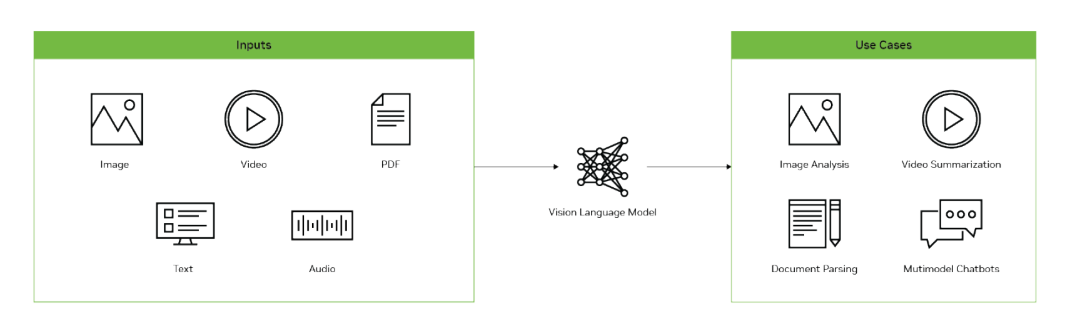
\includegraphics[width=\textwidth]{figures/VLM-example.png}
    \caption{视觉语言模型用例}
    \label{fig:vlm-example}
\end{figure}

\begin{figure}[htb]
    \centering
    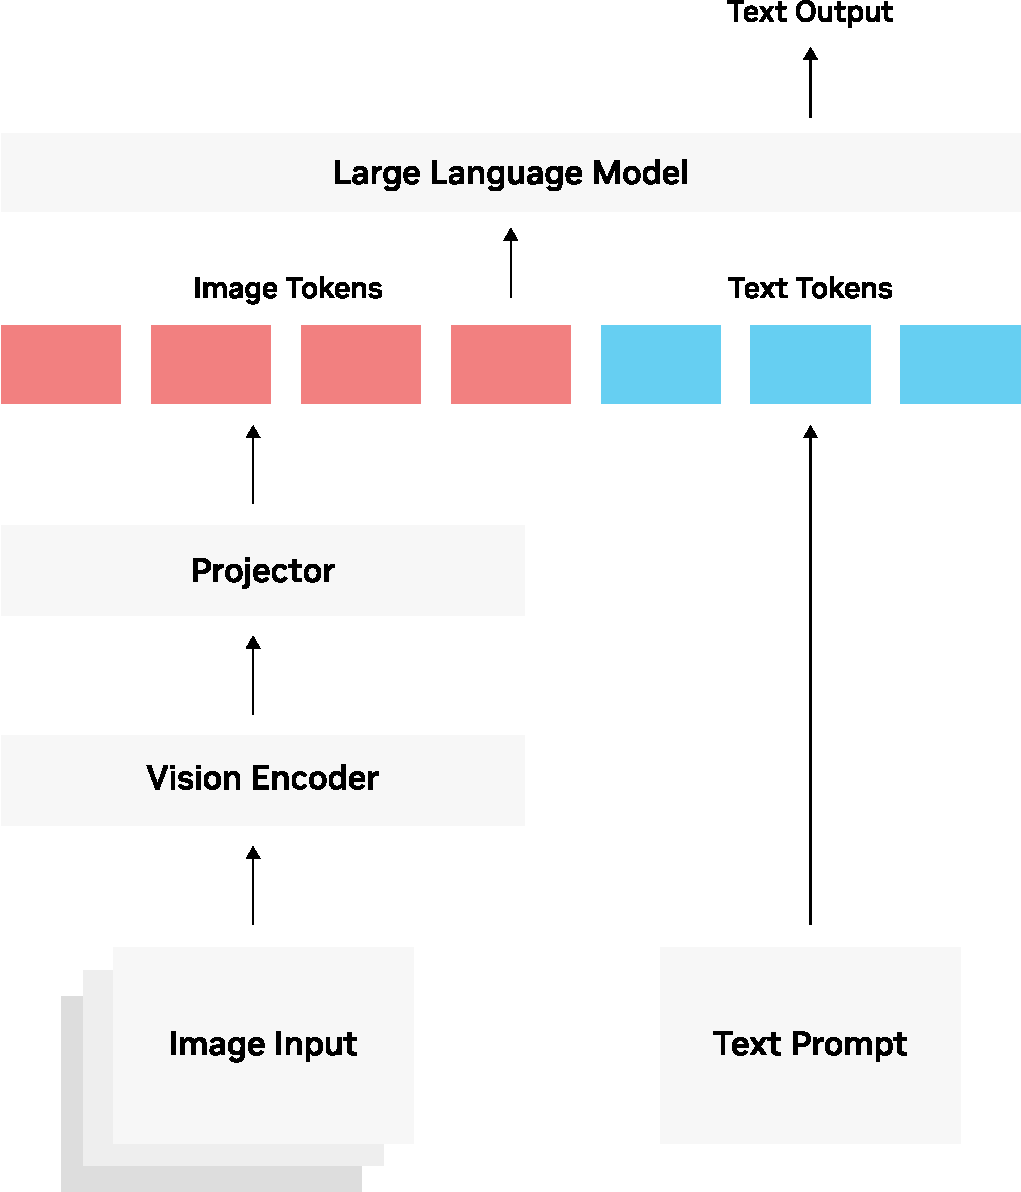
\includegraphics[scale=0.6]{figures/vlm-architecture-diagram-crop.pdf}
    \caption{视觉语言模型的通用三部分架构}
    \label{fig:vlm-architecture}
\end{figure}

尽管VLM在图像分类\cite{pratt2023does}、字幕生成\cite{alaluf2024myvlm}、
目标检测\cite{kuo2022f}、视频理解\cite{huang2024lita}和文档解析\cite{lv2023kosmos}
等各种任务中取得了良好效果,但VLM仍难以有效应对部分可见场景中基于空间推理的VQA任务。
部分可见指的是在图像中,某些物体或其特征由于遮挡、模糊、视野受限、噪声或其他原因而不可见的情况,
导致模型无法从图像中获得解决问题所需的全部信息。
现有的VLM在部分可见场景中解决VQA任务时,可能会出现幻觉\cite{vardi2025clipupclipbasedunanswerableproblem}
、空间关系推理能力下降\cite{chen2024spatialvlmendowingvisionlanguagemodels}\cite{anis2025limitationsvisionlanguagemodelsunderstanding}
,并且在对象识别和计数任务中表现不佳\cite{campbell2024understandinglimitsvisionlanguage},不能真正理解图像信息\cite{rahmanzadehgervi2025visionlanguagemodelsblind}等问题。
这类部分可见场景在现实世界中广泛存在,例如在机器人抓取、自动驾驶、安防监控等实际应用中,
系统往往需要在信息不完全的条件下对场景作出准确理解和决策。

因此,研究能够在部分可见场景中进行准确空间推理的VQA方法,不仅具有理论挑战性,也具有重要的工程价值。
一方面,它有助于提升人工智能系统在复杂环境中的稳健性和泛化能力;
另一方面,也为智能机器人\cite{gao2024physically}\cite{nasiriany2024pivot}、
AR/VR交互系统\cite{konenkov2024vr}等场景中的感知与决策提供了新的技术路径。

为了解决多模态模型在空间推理方面的问题,研究者们提出了一些新的方法。近年来,
神经符号方法(Neuro-Symbolic Methods)得到了广泛关注。在多模态空间推理场景中,
神经符号方法使用深度学习技术进行感知,为输入的图像和问题分别生成符号表示,再使用符号系统进行推理求解,
可以有效提升多模态模型在空间推理方面的能力。

在神经符号方法中,神经网络的选择十分多样,通常包括卷积神经网络(Convolution Neural Network, CNN)、
循环神经网络(Recurrent Neural Network, RNN)及其变体、图神经网络(Graph Neural Network, GNN)和
Transformer架构及LLM。相比其它神经网络,LLM用于神经符号系统,具有以下突出优势:
\begin{enumerate}[itemsep=0pt,parsep=0pt]
    \item 丰富的预训练知识库。LLM在大规模语料上进行预训练,具备广泛的世界知识和语言理解能力,这使得它们在处理涉及常识推理和多领域知识整合时,比专门针对单一任务训练的网络更具优势。
    \item 自然语言理解与生成能力。LLM能够将符号系统产生的抽象逻辑或规则,用自然语言进行解释和反馈,从而降低了人机交互的门槛,并使得系统的推理过程更易于理解和验证。
    \item 零样本/少样本学习能力。由于在大规模数据上学习到了通用的语言模式,LLM在面对新领域或数据较少的任务时,往往能够直接发挥作用,从而提高神经符号系统的泛化能力。
    \item 灵活的上下文建模。LLM能够捕捉长距离依赖和上下文信息,这对于将符号系统中离散的知识点进行有机整合,以及在复杂场景中实现动态推理具有重要意义。
\end{enumerate}
结合以上各项理由,将LLM作为神经符号系统中的神经模块,能够与符号系统形成互补,既利用符号逻辑的严谨性,又发挥神经网络在语义理解和自然语言生成方面的优势,从而构建更强大、更灵活的智能系统。

在神经符号方法中,符号系统的选择同样多种多样,例如知识图谱嵌入(Knowledge Graph Embeddings, KGE)、逻辑神经网络(Logical
 Neural Networks, LNN)都为信息表示和推理提供了新思路。其中,回答集编程(Answer Set Programming,ASP)也被
越来越多地采用作为符号系统。ASP是一种声明式编程范式,可用于解决复杂的人工智能问题,其起源于对逻辑编程、非单调推理和知识表示的研究。
相比其它符号系统,ASP被更多用于神经符号方法中,主要是由于以下几点优势:(1)明确的逻辑语义与可解释性。ASP基于严格定义的逻辑规则,其推理过程透明、易于解释。这一特性在需要精确推理和结果可验证的任务中尤为重要\cite{gelfond1988stable};
(2)强大的非单调推理能力。ASP自然支持非单调逻辑推理,能够处理默认情况和异常情形,这使其在面对现实世界中不完全或动态变化的信息时表现出色\cite{gelfond1988stable};
(3)成熟的求解器与工具支持。像Clingo这样的ASP求解器已经经过长期验证,具有高效、稳定的特点,能够处理大规模问题,这为实际应用提供了有力保障\cite{gebser2012answer};
(4)便于与神经网络等模块整合。ASP的声明式表达方式使其易于与神经网络输出的信息对接,形成互补优势,从而提升整体系统的推理能力\cite{garcez2002neural}。
ASP的这些特性使得它作为符号系统的杰出代表,被广泛应用于神经符号方法中。

尽管神经网络采用了预训练的LLM,而符号系统部分选用了ASP,但将二者有效结合在一起仍然是一项复杂的任务。
为此,近年来出现了一些神经符号框架,试图通过模块化设计和统一接口来简化LLM与ASP的集成开发流程\cite{wang2024dspybasedneuralsymbolicpipelineenhance}。
尽管现有的框架为LLM结合ASP的开发过程提供了诸多便利,降低了使用门槛,然而其在ASP规则的自动拓展方面存在不足,
需要依赖人工干预进行规则扩充,在这一方面仍存在改进空间。

为了测试模型解决空间推理问题的能力,涌现了诸如CLEVR、GQA、COCO等数据集。
这些数据集由问题答案对(Question and Answer Pair,以下简称QA对)组成,
并且包含问题对应的场景图像。CLEVR是一种积木世界的数据集,因其高度结构化的场景构造、精确标注的物体属性及复杂的空间关系,
而被广泛用于人工智能的研究和课堂教学等重要场景。
然而,CLEVR数据集图像均基于完整场景生成,所有回答问题的信息都直接可见,缺乏现实环境中常见的部分可见性,
难以有效考察VLM在部分可见场景中的推理能力\cite{sam-abraham-etal-2024-clevr}。
因此,要考察模型在部分可见积木世界中对空间推理问题的解答能力,需要对CLEVR进行改进,以使其具备部分可见性。

自动规划作为人工智能领域的一个重要分支,其核心目标是让计算机能够像人类一样,自主地制定实现特定目标的行动计划。
对能够完成积木世界中寻找、挪动物体等任务的智能体而言,空间推理显然是其能够完成任务指令的前置要求。
目前,市面上业已出现不少人工智能课程教学的演示系统,然而很少有演示教学系统
关注自动规划课程中的积木世界空间推理,不能展示智能体运用哪些知识以完成空间推理,进而达到最终目标。
为此,设计并实现一个自动规划课堂教学演示原型系统,展示智能体如何在部分可见的积木世界场景下完成空间推理,
对启发学生理解人工智能思考过程,进一步提升自动规划课程教学的可视化水平,具有十分重要的意义。

综上所述,积木世界作为空间推理研究的重要场景,虽在可视化、可控性和评估便利性方面具备显著优势,
但现有视觉语言模型在面对部分可见或遮挡场景时,其空间推理能力仍显不足。
神经符号方法通过引入形式化的逻辑推理机制,有效弥补了深度学习在可解释性和系统性推理方面的短板,
尤其是在复杂空间关系建模中展现出潜力。然而,当前神经符号VQA框架中ASP规则的拓展仍主要依赖于人工,
难以灵活适应动态环境和多样化任务需求。为进一步提升神经符号模型在部分可见场景中的空间推理性能,
亟需构建具挑战性的高质量数据集,并探索规则自动补充机制与大语言模型的协同方式,
从而推动视觉问答系统在积木世界场景中的智能推理能力发展,为自动规划课堂中教师向学生展示智能体如何理解外部环境信息并进行推理提供了便利。
\section{相关研究现状}
基于前述背景,本文的研究目标明确为:提升神经符号方法用于部分可见的积木世界的空间推理问答的准确率。
为达成该研究目标,所需了解的
研究领域包括VQA技术、VQA数据集、ASP程序生成、空间推理、神经符号方法在空间推理中的应用等。为此,本节将对这些领域的相关研究进行综述。
\subsection{VQA技术的研究现状}
VQA是由Antol等人\cite{Antol2015VQA}提出的,是人工智能领域中一个富有挑战性的交叉研究方向,
涉及计算机视觉(CV)、自然语言处理(NLP)和机器学习(ML)等多个学科。
其核心任务是让机器能够根据给定的图像内容和相关的自然语言问题,生成准确的自然语言答案。
VQA不仅要求模型理解图像中的视觉信息(如物体、属性、关系)和问题的语义意图,还需要进行复杂的推理,
融合这两种模态的信息来找到或生成答案。近年来,随着深度学习技术的发展,VQA领域取得了显著进展,但也面临着诸多挑战。

早期的VQA模型通常采用相对简单的框架,例如使用卷积神经网络(CNN)提取图像特征,使用循环神经网络(RNN)
或长短期记忆网络(LSTM)编码问题,然后通过简单的融合策略(如元素积、拼接)结合两种模态的特征,最后输入到一个分类器中预测答案。

然而,这类方法难以有效关联问题中的关键信息和图像中的特定区域。为了解决这个问题,注意力机制
被广泛引入VQA模型中。其核心思想是让模型根据问题的指导,动态地聚焦于图像中最相关的区域。其中, Anderson等人提出的自下而上的注意力机制\cite{anderson2018bottom}
成为后续许多模型的基础。该方法首先使用Faster R-CNN等目标检测器提取图像中的显著区域,
然后根据问题生成一个查询向量,计算该查询与各个区域特征的相似度(注意力权重),最后对区域特征进行加权求和,
得到与问题高度相关的视觉特征。这种方法显著提升了模型性能,因为它能更精确地定位与问题相关的视觉证据。
后续研究进一步发展了注意力机制,如分层注意力\cite{lu2016hierarchical}和共同注意力,后者允许模型同时学习图像区域和问题词语之间的相互关联,从而实现更深层次的跨模态信息交互。

随着Transformer架构在NLP领域的巨大成功,研究者们也开始将其应用于VQA任务,以更好地捕捉长距离依赖和模态间的复杂交互。
这些模型通常利用Transformer的自注意力和交叉注意力机制。ViLBERT\cite{lu2019vilbert}和 LXMERT\cite{tan2019lxmert}是早期的代表性模型。
它们采用双流架构,分别处理视觉和文本输入,并通过跨模态Transformer层进行信息交互和融合。VL-BERT\cite{su2019vl}和 Oscar\cite{li2020oscar}则采用了单流架构,
将图像区域特征和文本词嵌入拼接在一起,输入到一个统一的Transformer编码器中进行联合建模。Oscar还引入了目标标签作为“锚点”,
连接图像区域和对应的文本描述,增强了跨模态对齐。

这些基于Transformer的视觉语言预训练(Vision-Language Pre-training, VLP)模型通常在大规模的图像-文本对数据上进行预训练,
学习通用的跨模态表示,然后在特定的VQA数据集上进行微调,取得了显著的性能提升。

近年来,LLM如GPT-3、PaLM等在自然语言处理任务上展现了惊人的能力。
研究者们迅速探索了将LLM应用于VQA领域,催生了大型多模态模型(Large Multimodal Model, LMM) 或 
VLM的研究热潮。这类模型通常利用预训练好的强大LLM作为基础,通过设计特定的接口或适配器将视觉信息“注入”到LLM中,使其能够理解图像内容并回答相关问题。
OpenAI发布的GPT-4V\cite{openai2023gpt4v}展示了前所未有的多模态理解和推理能力,
能够处理复杂的视觉问答、图像描述、图表解读等任务。虽然其具体架构和训练细节未完全公开,但它代表了当前LMM能力的顶尖水平。

基于LLM的VQA模型通常具有更强的零样本/少样本泛化能力、更自然的语言交互能力、更好的常识推理能力,
并且能够处理更开放式、更复杂的查询。它们将VQA从一个多模态分类/生成任务,转变为一个基于视觉信息的条件语言生成任务。

尽管VQA领域取得了巨大进步,但仍面临一些挑战。
第一是深度推理与组合性。模型在处理需要多步逻辑推理、精确计数或复杂空间关系的问题时仍然困难。
第二是鲁棒性与偏见。模型容易受到对抗性样本攻击,并且可能学习到数据集中的统计偏见,而非真正的视觉理解。
第三是可解释性。理解模型为何给出特定答案仍然是一个挑战,尤其对于复杂的黑箱模型。
第四是知识依赖。如何更有效地融合和利用外部世界知识或领域知识来回答专业性或常识性问题。
第五是效率与部署。大型多模态模型通常计算量巨大,如何在资源受限的设备上高效部署是一个实际问题。
\subsection{VQA数据集的研究现状}
VQA作为跨模态推理的重要任务,近年来在VQA数据集建设方面取得了显著进展。
早期的VQA v1.0与v2.0数据集主要基于真实图像,问题类型以事实性提问为主,虽然具备一定规模,
但在逻辑推理深度和场景可控性方面存在明显局限。因此,研究者逐步转向使用合成图像生成更具可控性和推理复杂度的数据集,
以更有效地评估模型的逻辑与空间推理能力。

CLEVR\cite{johnson2017clevr}是该方向中的代表性数据集,被广泛用于评估模型在属性识别、比较、空间关系理解等方面的能力。
该数据集通过精心设计的合成场景和程序化生成的问题模板,有效规避了偏差问题,同时提供了清晰的程序标注,
使其成为神经符号推理方法的标准测试平台。尤其在空间关系理解方面,CLEVR提供了诸如“左边的球是什么颜色?”、
“与红色立方体相邻的物体有多少个?”等类型的问题,涵盖了多种空间方位与拓扑关系,为开发具备空间推理能力的模型提供了重要实验基础。

本文课题以积木世界为背景,而CLEVR数据集在任务设定和场景设计上,与积木世界有高度相似性:
同样使用规则几何体组合构建三维场景,并注重问题的组合推理特性。
因此,CLEVR不仅为本文提供了可借鉴的数据构造方法,也验证了基于合成场景推动空间推理研究的有效性。

然而,CLEVR在设计上假设场景信息完全可见,即观察者可以从固定角度完整获取所有物体的属性与相对关系。
这种全可见性的假设简化了推理难度,却与现实环境中部分可见场景存在显著差异。部分可见性常见于机器人导航、现实场景感知等任务中,
在这种情况下,模型不仅要理解空间关系,还需在不完全信息下进行补全与推断。
此外,CLEVR并不要求模型在回答问题时主动使用图像场景以外的背景知识或逻辑约束,模型主要使用对图像内容的直接理解
和内部逻辑进行推理,并不能充分考察模型利用现有常识进行推理的能力。
由此看来,CLEVR虽然在空间推理研究中奠定了坚实基础,
但仍难以满足部分可见积木世界的问答任务的需求。

因此,以CLEVR数据集为基础,将部分可见性引入CLEVR数据集,对研究部分可见的积木世界中的空间推理问答任务具有重要意义。
\subsection{生成ASP程序的研究现状}
本研究旨在提升神经符号方法在部分可见的积木世界空间推理问答任务中的准确性,其中ASP程序的自动生成能力是关键组成部分之一。
积木世界中的空间问答不仅要求模型理解图像中的空间结构并生成对应的逻辑程序,还需将自然语言问题转换为逻辑形式进行推理。
在这一过程中,如何高效、准确地生成ASP代码,直接影响到神经符号系统的整体推理效果与任务完成度。
以下将对当前自动生成ASP程序的研究现状进行综述。

近年来,代码自动生成技术在学术界和工业界均得到了广泛关注与深入研究。
已有研究表明,自动合成程序具有显著的效率与准确性优势 \cite{ernst2022ai}\cite{peng2023impact}\cite{dakhel2023github},
并已广泛应用于几乎所有主流的命令式编程语言中 \cite{chen2021evaluating}。
其中,大型语言模型(LLMs)作为核心技术手段,在代码生成任务中表现出了极强的能力,并在多个基准测试中得到了系统性的评估 \cite{xu2022systematic}\cite{wang2023codet5+}。同时,也有研究指出,通过针对特定任务微调模型可以进一步提升其在命令式语言代码生成中的表现 \cite{ma2024llamoco}。

在声明式编程领域,尤其是针对答案集程序设计(Answer Set Programming, ASP)的自动生成,
同样引起了研究者的广泛关注。相关研究主要致力于构建工具,自动将自然语言规范转换为ASP程序,
以缩短自然语言表达与逻辑程序之间的语义距离 \cite{erdem2009transforming}\cite{fang2017approach}\cite{schwitter2018specifying}\cite{caruso2024cnl2asp}。早期的研究主要集中于将简化英语表述的逻辑谜题自动转化为ASP程序,通过λ演算与概率组合范畴语法等方法进行语义解析 \cite{baral2012solving}。

随后,研究者提出了“受控自然语言(Controlled Natural Languages, CNLs)”的概念,
用于在保留自然语言可读性的同时,满足逻辑编程所需的形式化表达要求 \cite{kuhn2014survey}。
Erdem等人提出了BIOQUERYCNL语言并给出了其向ASP查询语句转译的算法 \cite{erdem2009transforming};
Fang等人基于LANA注解机制,设计了一套适用于SeaLion IDE的CNL构造方案 \cite{fang2017approach};
2018年,Schwitter开发了PENGASP语言,用于ASP程序的语言化与可视化表达 \cite{schwitter2018specifying}。
近年来,Dodaro等人推出的CNL2ASP工具实现了从CNL到ASP的自动转换,并已公开发布,成为该领域的一项重要成果 \cite{caruso2024cnl2asp}。
尽管CNL显著降低了ASP的使用门槛,为非专业用户提供了更为自然的表达方式,
但其语法与词汇依然受到约束,仍然要求用户具备一定的形式化语言构造能力,限制了其普适性与灵活性。

随着大型语言模型的发展,研究者开始尝试将其与ASP系统相结合,从而在自然语言理解与逻辑推理之间建立更直接的连接。
Nye等人提出的“双系统模型” \cite{nye2021improving},利用GPT-3生成自然语言语义解析器,并与ASP推理模块进行集成,
显著提升了系统的推理能力与泛化性能。
Yang等人进一步验证了GPT-3作为少样本语义解析器的可行性,
能够在无需专门微调的情况下将自然语言问题直接转化为ASP格式的逻辑表达 \cite{yang2023coupling}。
此外,Ishay等人结合提示工程技术,基于Mitra等人的逻辑谜题数据集,构建了ASP自动求解系统 \cite{mitra2016addressing};
Rajasekharan等人则在STAR框架中系统性地实现了LLMs与ASP的结合,用于多种自然语言理解任务 \cite{rajasekharan2023reliable}。

尽管已有研究已初步展示了LLMs在ASP生成方面的潜力,但系统性面向声明式语言(特别是ASP)代码生成的研究仍较为匮乏。
2024年,Borroto等人提出并实现了NL2ASP工具 \cite{borroto2024automaticcompositionaspprograms},该工具基于两阶段架构:
首先通过神经机器翻译模型(如T5-small、Bart-base)将自然语言转换为受控自然语言形式;随后借助CNL2ASP工具生成对应的ASP程序。
该方法在图结构类问题中展现出较好效果,是将LLMs用于ASP程序自动生成的重要探索之一。

然而,NL2ASP方法仍存在诸多限制:其一,其适用范围主要集中在图相关问题,通用性较弱;
其二,采用中间表示形式(CNL)增加了系统复杂性,可能引入额外的误差与信息损失;
其三,虽然作者指出了LLMs在ASP代码生成中的低表现,但尚缺乏系统性、全面的实证分析。

综上所述,当前针对ASP程序的自动生成研究已取得初步进展,
从早期的受控自然语言设计到近年来结合大语言模型(LLMs)进行语义解析与代码合成,相关技术不断演进。
以上这些研究为进一步提升ASP程序自动生成的准确率,拓展ASP的应用范围并提升神经符号方法在积木世界空间推理问答任务中的表现提供了
研究空间与创新方向。
\subsection{空间推理的研究与现状}
空间推理涉及对物体位置、方向、距离以及相互关系的理解和处理,是计算机视觉、自然语言处理以及机器人导航等领域的核心能力。
尽管人类在空间推理上有天然优势,但当前的模型(尤其是大语言模型和视觉语言模型)在这方面仍面临不少挑战。
这一问题催生了大量针对空间推理能力提升的研究工作。

基于规则的符号推理最早被用于解决空间推理问题,其核心思想是使用几何约束(如欧氏距离、拓扑关系RCC8)和逻辑推理(如谓词逻辑)建模空间关系。
Allen等人提出了相关方法。然而,这种方法过于依赖人工规则,难以处理复杂场景和非结构化数据,实际应用价值有限。后来,有一部分研究者将概率图模型引入到空间推理问题中。
Kuipers等人提出空间语义层次模型,结合贝叶斯网络或马尔可夫随机场(MRF)建模空间关系的不确定性。

进入2010年代,深度学习方法开始快速发展,一些研究者将深度学习方法引入空间推理领域。Antol等人\cite{Antol2015VQA}提出使用CNN+LSTM直接预测
空间问题的答案,Xu等人\cite{xu2017scene}提出使用场景图生成的方法检测物体及其空间关系。这些端到端神经网络的方法,都是黑箱模型,缺乏可解释性,且易受数据偏差影响。
后来有研究者尝试使用图神经网络解决空间推理问题,将场景建模为图结构,通过消息传递捕捉空间关系。

2023年,以OpenAI的ChatGPT广受世界关注为标志,LLM得以迅速发展。以LLM为重要组成部分的VLM得以快速发展,应用于空间推理问题的解决中。
研究者致力于增强VLM的空间推理能力,取得了一系列重要成果。
例如,Google DeepMind开发的SpatialVLM\cite{chen2024spatialvlmendowingvisionlanguagemodels}项目通过生成并训练一个大规模3D空间视觉问答(VQA)数据集,
显著提升了VLM在空间推理任务中的表现。该研究利用互联网规模的真实世界图像,自动标注了约1000万张图像和20亿个VQA示例
(其中50\%为定性,50\%为定量),在二元谓词预测任务中达到了75.2\%的准确率,远超GPT-4V(68.0\%)和LLaVA-1.5(71.3\%)。
此外,SpatialVLM在定量问题中输出数字的比率达到99.0\%,其中37.2\%的答案落在[50, 200]\%的范围内,展示了其在链式思维空间推理和机器人应用中的潜力,
如为机器人任务提供密集奖励注释。

另一项研究SpatialRGPT\cite{cheng2024spatialrgptgroundedspatialreasoning}通过引入数据整理管道和灵活的“插件”模块,
整合深度信息到视觉编码器中,增强了VLM在3D空间认知中的表现。该研究提出了SpatialRGBT-Bench基准,包含室内、外和模拟环境的3D注释,
用于评估VLM在复杂环境下的空间推理能力。这些进展表明,通过大规模数据训练和多模态信息整合,VLM的空间推理能力得到了显著提升。

尽管VLM在空间推理任务中取得了一定的进展,但VLM仍在部分可见场景中存在一些局限性,主要体现在以下几个方面:
\begin{enumerate}[itemsep=0pt,parsep=0pt]
\item 幻觉现象。当视觉信息不完整时,VLM 往往会生成不正确或虚构的答案,
即“幻觉”出图像中不存在或无法从可用视觉线索中可靠推断出的细节。这种趋势在问题涉及完全缺失的对象时可能尤为明显,
尽管模型对答案充满信心,实际上却给出了错误答案\cite{vardi2025clipupclipbasedunanswerableproblem}。
\item 空间关系推理能力下降。理解对象之间如“后面”或“旁边”的空间关系通常依赖于完整或足够的视觉线索。
当场景中的某些部分由于遮挡或视野受限而缺失时,VLM对空间关系的准确辨识能力会受到严重影响,甚至出现逃避或胡乱回答的现象\cite{chen2024spatialvlmendowingvisionlanguagemodels}。
\item 部分基本任务出现失败。有研究指出,在部分可见场景下VLM在一些基本的多对象推理任务(如计数和定位)上的表现不佳\cite{campbell2024understandinglimitsvisionlanguage}。
\end{enumerate}

这些局限性表明,当前基于LLM的VLM仍难以有效应对基于空间推理的VQA任务,特别是在出现遮挡、视野受限、噪声等情形的部分可见场景中。
\subsection{神经符号方法应用于空间推理中的研究现状}
为克服上述局限,研究者开始探索神经符号方法,将神经网络的模式识别能力与符号推理的逻辑表达能力相结合。
神经符号方法通过显式表示空间关系和逻辑规则,能够更好地处理复杂推理任务,尤其是在多跳推理和泛化能力方面。

最早将神经符号方法用于空间推理的工作是由Andreas等人\cite{andreas2016neural}提出的Neural Module Network(NMN),其核心思想是:NMN通过模块化分解,将复杂推理拆解为可复用子模块的动态组合,
使模型能根据问题语义动态调整计算路径。最终在CLEVR数据集上实现了超过90\%的准确率,显著优于传统的CNN-LSTM模型。这一开创性的工作,为
后续神经符号推理的研究奠定了基础。

Yi等人\cite{yi2019neuralsymbolicvqadisentanglingreasoning}在Andreas等人的工作基础上,提出了Neural-Symbolic VQA(NS-VQA)模型,
通过设计神经符号解耦框架,将视觉感知、语言理解和符号推理解耦,以减少跨模态耦合带来的偏差放大效应,并通过符号程序将问题转化为可执行的推理步骤,避免端到端模型对语言表面模式的依赖。
最终实验结果表明,NS-VQA在CLEVR数据集上达到了94.5\%的准确率,验证了神经符号方法在空间推理中的有效性。此外,NS-VQA通过分离语言理解和视觉推理,模型对语言分布偏移的敏感性降低,性能提升约15\%。
该成果是神经符号融合的样板性工作,首次在VQA中系统整合符号推理与深度学习,为后续神经符号AI研究提供方法论基础,也为对抗语言先验提供了一种解决方案,
推动VQA从“模式匹配”向“真实理解”演进。

后续,Yang等人\cite{yang2020neurasp}提出了NeurASP这类方法在 NS‐VQA 的基础上引入了神经原子(neural atom)和选择规则,
用以更灵活地处理对象检测的不确定性,缓解了对强监督程序注释的依赖,并在一定程度上改善了符号执行模块的透明性。Thomas等人\cite{eiter2022neuro}对NeurASP中进行改进,在ASP编码和不确定性管理上采用了基于统计门槛的筛选策略,
致力于提高系统的效率和鲁棒性,同时更明显地解耦视觉感知与符号推理,使得推理过程更加透明和可解释。

随着LLM在2023年的迅速发展,越来越多的研究者将LLM引入到神经符号方法中,取代传统的CNN、RNN、LSTM等神经网络。Bauer\cite{bauer2023neuro}等人
利用大型语言模型(LLMs)进行语言解析,相比传统的 LSTM 或其他序列模型,LLMs 能够更准确、灵活地将自然语言问题转化为符号化的查询或图结构表示。这不仅提高了程序生成的质量,还增强了对复杂语言结构和多样化问句的处理能力,实现了神经和符号推理模块的更深层次融合。

尽管将LLM引入神经符号方法后,一系列实验证明LLM在空间推理方面表现不俗,但仍存在一系列问题。
Wang等人\cite{wang2024dspy}在研究中指出,LLM通常只能捕捉语义信息,对于需要精确定义物体位置、方向、距离等空间关系的问题,经常出现理解不足或错误推理。
此外,在需要连续、层次化空间推理的任务中,LLM容易失去推理链条,导致答案不连贯或不准确。另外,
直接通过自然语言生成逻辑代码(例如ASP规则)时,LLM容易生成语法或逻辑不一致的输出,从而使整个推理流程失效。
针对这些问题,他们提出了一个基于DSPy的神经符号管道。
该管道使用LLM将自然语言描述转化为符号化表示(事实和规则),而将具体的逻辑推理任务交给回答集编程(ASP)模块处理,并且利用DSPy框架,通过多轮反馈和自我修正
,改进LLM生成的ASP代码,降低解析错误、变量绑定错误等问题,提高ASP代码的可执行性。
另外,其将LLM在自然语言理解上的优势与ASP在逻辑推理上的精确性相结合,从而在如StepGame和SparQA等空间推理任务上大幅提升准确率。

Wang等人\cite{wang2024dspy}的工作展示了神经符号方法在空间推理中的潜力,大大简化了ASP与LLM进行系统集成的难度,充分发挥了LLM和ASP各自的优势,
为这神经符号方法在空间推理领域的普及做出了积极贡献。然而,其提出的神经符号管道仍然存在一些局限性,
主要体现在不能实现对ASP规则的自动拓展。在每次推理完成后,ASP求解器产生的答案集,可能会包含一些新的事实或规则。而现有的神经符号管道并不能自动将这些新产生的事实或规则反馈存放到本地ASP知识库中,
进而无法利用过去的推理经验来提升后续推理的效率和准确性。
对神经符号管道的进一步改造,可以围绕以上的问题进行进一步深入研究。

总的来看,神经符号方法在空间推理领域展现了强大的潜力,特别是在语言驱动、视觉驱动和机器人应用中。尽管当前存
在挑战,但其在组合性推理和可解释性方面的优势为AI系统的进一步发展提供了重要方向。
随着研究的深入,神经符号方法有望在更广泛的现实世界应用中发挥作用。
\subsection{人工智能课程教学演示系统的研究现状}
人工智能作为第四次工业革命的驱动因素,业已成为世界各国的关注焦点,而培养人工智能的相关人才自然而然也
成为学校和各级教育部门的工作重点。我国政府高度重视人工智能在教育中的应用,制定了一系列政策以推动人工智能教育的发展。
​教育部提出到2030年前在中小学基本普及人工智能教育,强调构建系统化课程体系、实施常态化教学与评价、开发普适化教学资源等六大任务。\cite{moe_ai_2024}

目前,关于人工智能课程的相关教学工具大致分为以下几类:
\begin{enumerate}[itemsep=0pt,parsep=0pt]
\item 
\end{enumerate}

自动规划作为人工智能领域的一个重要分支,其核心目标是让计算机能够像人类一样,自主地制定实现特定目标的行动计划。
积木世界作为一个由规则几何体构成的场景,能够很好地满足自动规划课程的入门教学需要,能够简单、直观地让学生快速
把握智能体所在的环境,方便学生对相关空间推理问题进行思考。
对能够完成积木世界中寻找、挪动物体等任务的智能体而言,空间推理显然是其能够顺利完成人类下达的任务指令的前置环节,
是高阶人工智能完成复杂任务的前置阶段。引导学生理解智能体如何基于先验知识和积木世界中的环境信息做出决策,
是自动规划课程教学中十分重要的教学目标,对人工智能的初阶教学具有重要意义。
然而,当前很少有关注自动规划课程的教学演示系统。通过回答积木世界中的空间推理问题,并展示推理所使用的相关规则、知识
,能够更好地让学生理解智能体的思考过程,提高教学的可视化水平,进而启发学生更深入理解人工智能的内在逻辑,
提高学生的人工智能素养。

因此,开发一款自动规划课堂教学演示系统,能够完成积木世界的空间推理问答并展示思考过程,对于自动规划课程的
入门教学以及提高学生的人工智能素养,具有十分重要的意义。
\section{研究思路}
基于前述研究背景,本课题的主要研究目标是:
提出一种新的神经符号VQA框架,使其支持对ASP规则进行自动扩展,进而丰富空间推理可用的规则并减轻开发人员手动补充ASP规则的负担,
并通过实验验证新设计的神经符号VQA框架能够有效提升部分可见积木世界场景下的空间推理问答的准确率。

根据上述主要研究目标,结合前述相关研究现状,本文决定围绕以下几个方面展开工作:
\begin{enumerate}[label=(\arabic*),itemsep=0pt,parsep=0pt]
\item 针对当前CLEVR数据集中场景完全可见、不要求模型使用外部知识或逻辑规则进行推理的问题,
本文对CLEVR数据集进行改进,引入部分可见性并使用ASP定义环境约束,构建积木世界空间推理数据集,
以评估模型在部分可见的积木世界场景下,能否主动利用外部背景知识或逻辑规则,对正确回答用户提出的积木世界空间推理问题。
\item 针对现有神经符号VQA框架不能自动根据已有知识拓展推理过程中所需ASP规则的问题,
本文提出一种新的神经符号VQA框架,使用大语言模型自动对知识库中选出可用于补充的ASP规则,
充实空间推理过程中所用ASP规则,从而实现对ASP规则的自动拓展能力
,减少ASP规则拓展过程中对人工的依赖,
并通过实验证明该框架能够有效提升VQA系统在部分可见积木世界场景下的空间推理问答的准确率。
\item 针对自动规划课程教学中可视化教学水平有待进一步提高的问题,本文基于所设计的神经符号VQA框架,
实现一个自动规划课堂教学演示原型系统。
该系统支持在自动规划课程的授课场景下,由教师向系统提出积木世界的空间推理问题,
系统进行解答并展示推理的中间步骤和逻辑链条,
为教师向学生形象展示智能体如何理解外部环境信息并进行推理提供了便利。
\end{enumerate}

图\ref{plan}对本文的研究目标、对应所需解决的关键问题、研究内容与研究产出进行了总结。
\begin{figure}[h]
    \centering
    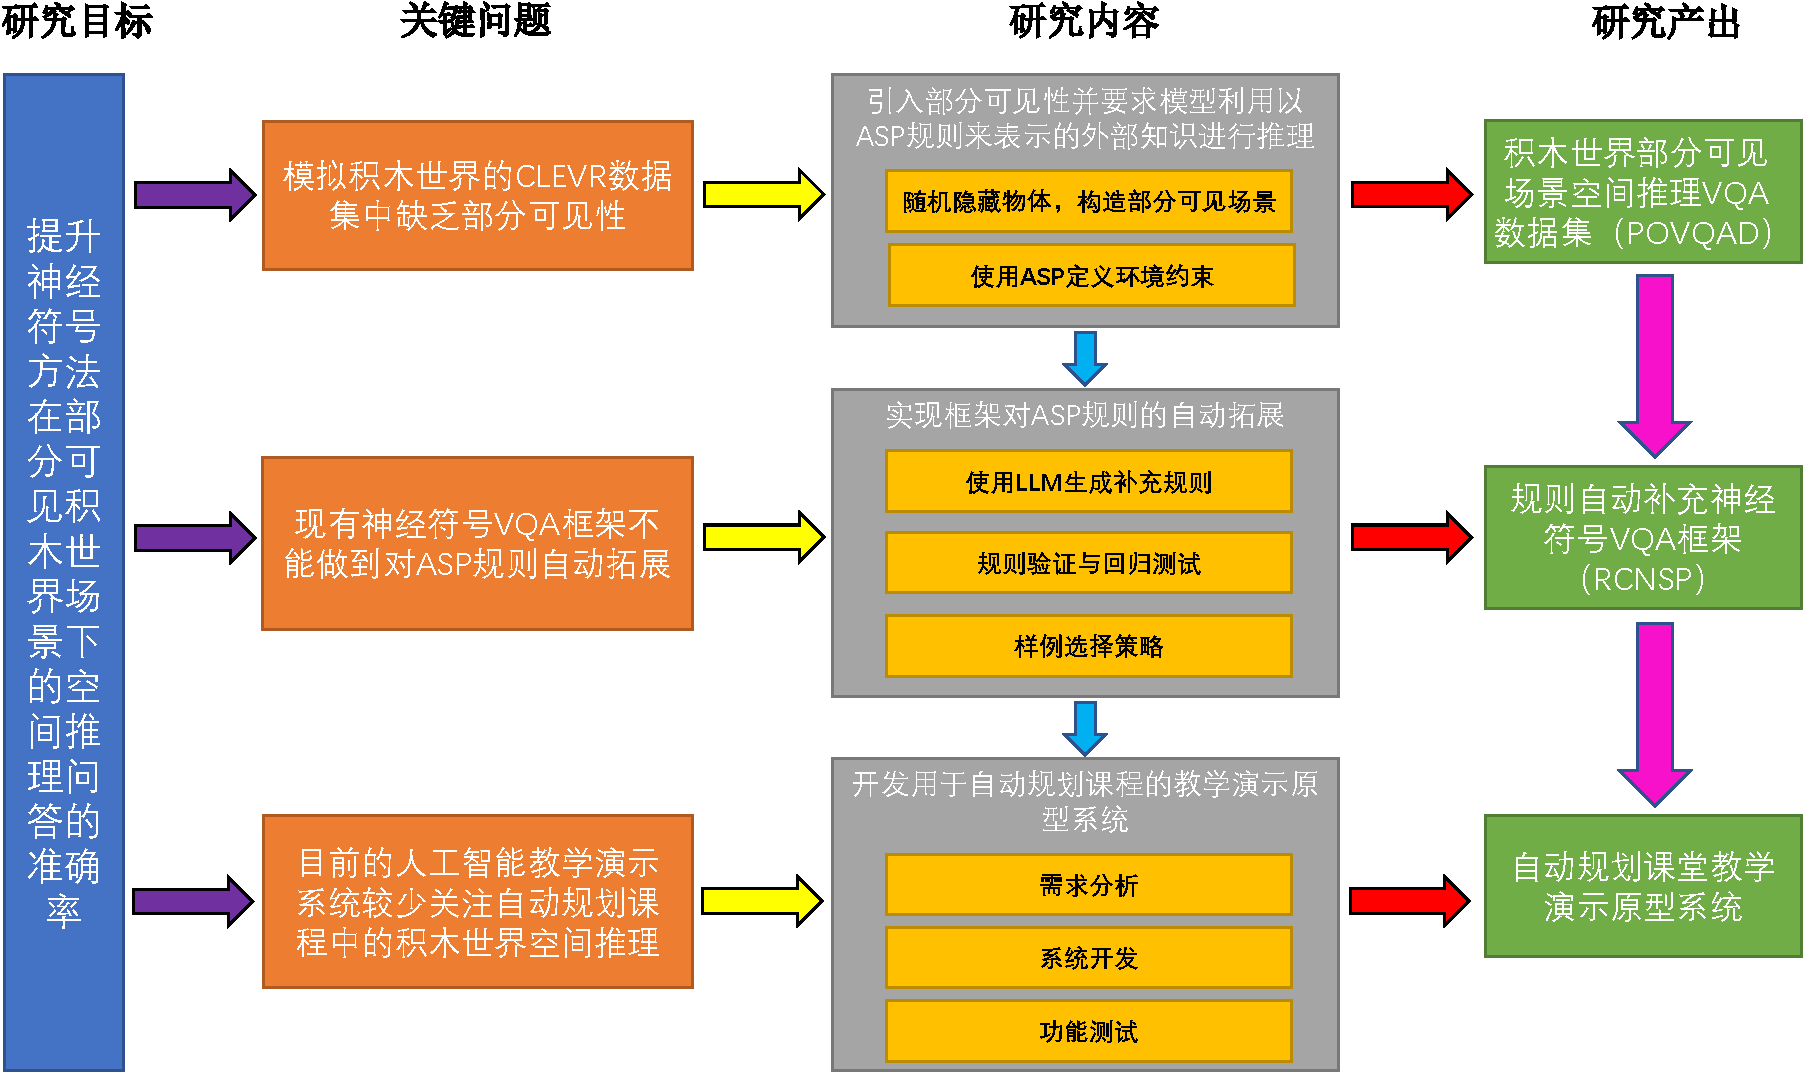
\includegraphics[width=\textwidth]{figures/research-guideline-crop.pdf}
    \caption{研究计划}
    \label{plan}
\end{figure}
% \begin{figure}[h]
%     \centering
%     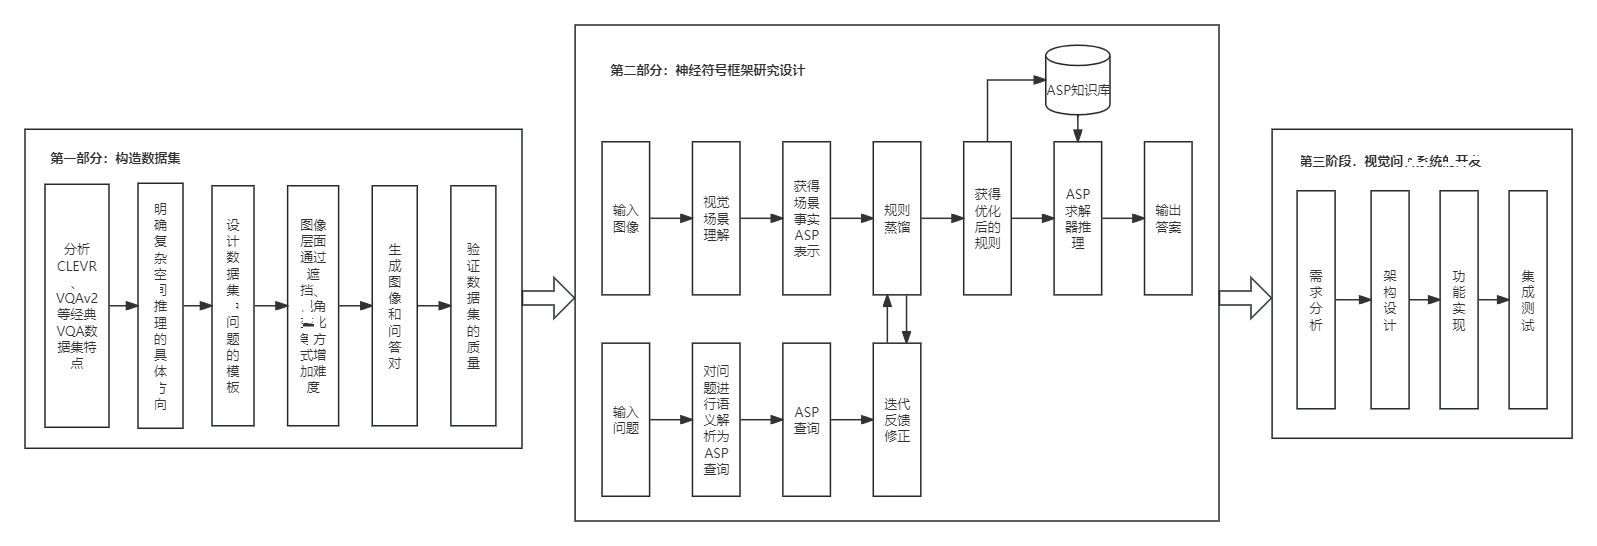
\includegraphics[width=\textwidth]{process.png}
%     \caption{技术路线图}
%     \label{roadmap}
% \end{figure}
\section{论文结构}
本文共分为六个章节,各章节的主要内容具体如下:

第一章为绪论,总体介绍本文的研究背景及意义、相关研究现状、研究思路及本文的结构安排。

第二章为背景知识,对本文涉及到的主要技术进行介绍,具体包括CLEVR数据集、ASP程序语法及ASP求解器、
GLIP以及DSPy。

第三章为数据集构建。对本文所用的视觉问答数据集进行详细介绍,
包括数据集的构造目的、数据集的研究方向、数据集的设计流程以及对数据集质量的验证。

第四章为神经符号VQA框架的研究设计。本章详细介绍本文设计的神经符号VQA框架,
包括总体架构、视觉场景理解、语义解析、知识蒸馏、迭代反馈、规则修正和 ASP 推理等模块,并通过对比试验证明了相比于VLM直接问答,神经符号方法能够有效提升模型在部分可见场景
下回答空间推理问题的正确率,并证明了本文新增的知识蒸馏模块能够进一步提升神经符号方法解决空间推理任务时的性能。

第五章为问答系统的设计与实现。对本文设计的VQA课堂教学演示原型系统进行详细介绍
,包括系统需求分析、系统架构设计、模块划分、模块实现和系统集成等内容。

第六章中对本文工作加以总结,分析本文的创新点和不足之处,并对未来的研究方向进行展望。


\newtheorem{definition}{定义}[section]
\newtheorem{example}{例}[section]
\chapter{背景知识}
\section{回答集编程}
% \numberwithin{equation}{section}
\subsection{语法}
项(terms)是ASP程序中最基本的元素,项可以是常量、变量或者函数。常量以符号常量或者数字表示(如4、a)。变量以字符串来表示,
要求首字母必须大写(如Dog、Person)。函数由函数符号与若干参数构成,例如$f(t_1,...,t_n),(n \geq 0)$。各参数
$t_i,(i=1,2,...,n)$也是项。若项中不存在函数符号与变量,则称该项为实例化项,否则称该项为非实例化项。

原子(atom)由谓词和项共同组成,例如$q(t_1,...,t_n),n \geq 0$。其中,$q$为$n$元谓词的标识符,$t_1,...,t_n$为项,
$n$为0时,谓词之后的括号可以省略。原子用于表示不同项之间的关系,例如:$dog(animal)$、$family(jensen,lucy)$、
$tomorrow\_sunny$,分别表示狗是动物、jensen和lucy是家人以及明天晴天。如果原子中的每一项都是实例化的,则该原子是实例化
原子,否则,该原子是非实例化的原子。例如,$dog(animal)$是实例化原子,$family(jensen,lucy)$是非实例化原子。
原子$q(t_1,...,t_n)$的强否定形式为$\urcorner q(t_1,...,t_)n$,其中符号$\urcorner$是经典逻辑中的否定,
$\urcorner q(t_1,...,t_n)$表示各项$t_i(1 \leq i \leq n)$。不符合
$q$所描述的关系,$\urcorner \urcorner a = a$,与经典逻辑中的排中律相同。文字(literal)可以是原子
$q(t_1,...,t_n)$,也可以是原子的强否定形式$\urcorner q(t_1,...,t_n)$。若文字对应的原子是实例化的,则称
该文字是实例化的。

\begin{definition}[规则] 规则$r$是具有如下形式的式子:
    \begin{equation}
        l_0 \thinspace or ... \thinspace or \thinspace l_m \leftarrow l_{m+1},...,l_n \thinspace not \thinspace l_{n+1},...,\thinspace not \thinspace l_p.
    \end{equation}
\end{definition}

其中$p \ge n \ge m \geq 0, l_i$代表文字,$not$为新的逻辑连接符,通常称作缺省否定符(default negation)或者
失败即否定(Negation As Failure, NAF),又称为若否定,$not \thinspace l_i$被读作“没有理由相信$l_i$为真”,但是这并不表明
$l_i$为假。对ASP程序而言,$not not a$不与a等价。规则r读作“如果相信$l_{m+1},...,l_n$为真,并且没有理由相信
$l_{m+1},...,l_p$为真,则相信$l_0 \thinspace or \thinspace ... \thinspace l_m$为真”。将$not l_i$称为缺省
文字(default literal),文字与缺省文字共同组成拓展文字(extended literal)。

规则$r$左侧的文字称为头部,可以表示为$head(r) = \{ l_0,...,l_m \}$。规则$r$右侧的文字称为体部,可以表示为
$body(r) = \{ l_{m+1},...l_n,not \thinspace l_{n+1},..., not \thinspace l_p \}$,规则的体部可以分为正
体部与负体部,正体部表示为$body^+(r) = \{ l_{m+1},...,l_n \}$,负体部表示为$body^-(r)=\{ l_{n+1},...,l_p \}$
。因此,规则$r$可以表示为:
\begin{equation}
    head(r) \thinspace \leftarrow \thinspace body^+(r), \thinspace not body^-(r) \label{con:body}
\end{equation}
一个ASP程序是有限条\eqref{con:body}所示的规则组成的集合。根据规则各部分所满足的相关条
件,可以分别定义事实、约束、正规规则、缺省规则和严格规则,如定义\eqref{def:fact}-定义\eqref{def:definite_rule}所
示。

\begin{definition}[事实]
当规则$r$满足$head(r)\neq \emptyset, body(r) = \emptyset$时,被称为事实(fact)。\label{def:fact}
\end{definition}
\begin{definition}[约束]
当规则$r$满足$head(r)= \emptyset, body(r) \neq \emptyset$时,被称为约束(constraint)。
\end{definition}
\begin{definition}[正则规则]
    当规则$r$满足$|head(r)|=1$时,被称为正则规则(normal rule)。
\end{definition}
\begin{definition}[缺省规则]
    当规则$r$满足$body(r)^-\neq \emptyset$时,被称为缺省规则(default rule)。
\end{definition}
\begin{definition}[严格规则]
    当规则$r$满足$body(r)^- = \emptyset$时,被称为严格规则(definite rule)。\label{def:definite_rule}
\end{definition}
根据上述各类规则的定义,本文进一步定义简单逻辑程序、缺省逻辑程序和正规逻辑程序如下。
\begin{definition}[简单逻辑程序]
    若程序$P$由有限条严格规则组成,则$P$被称为简单逻辑程序。
\end{definition}
\begin{definition}[拓展逻辑程序]
    若程序$P$由有限条缺省规则组成,则$P$被称为拓展逻辑程序。
\end{definition}
\begin{definition}[正则逻辑程序]
    若程序$P$除约束外,由有限条正则规则组成,则$P$被称为正则逻辑程序(Normal Logic Program, NLP)。
\end{definition}
若不做特别说明,本文考虑的程序均为不含约束的正规逻辑程序,即程序中的每条规则头部有且仅有一个文字。
\subsection{语义}
\subsubsection{文字的可满足性语义解释和程序的模型}
作为基础理论,首先给出 Herbrand 域、Herbrand 基的定义,分别如定义2.10和2.11所
示,进一步定义规则与程序的实例化,最终在实例化程序下讨论文字的可满足性语义解
释和可满足性。
\begin{definition}[Herbrand基]
    $P$是一个 ASP 程序,将程序$P$中出现的常量和函数形成的
    所有不含变量的项的集合称为 Herbrand 域,使用$\mathcal{U}_P$表示。
\end{definition}
\begin{definition}[Herbrand域]
    $P$是一个 ASP 程序,出现在程序$P$的规则中的谓词符号与
$\mathcal{U}_P$中的项组成的所有可能的不含变量的原子集合称为程序$P$的 Herbrand 基,使用$\mathcal{A}_P$
表示,为了保持简洁,通常简写为$\mathcal{A}$。
\end{definition}
\begin{definition}[规则的实例化]
    给定$P$中的一个规则$r$,使用$ground(r)$表示通过使用
$\mathcal{A}_P$中的常量对应地替换$r$中变量而获得的规则集合,这一映射被称为规则的实例化。
\end{definition}
\begin{definition}[程序的实例化]
    程序$P$由一系列规则的集合组成,程序$P$的实例化$ground(P)$表示为式\eqref{equation:ground}:
    \begin{equation}
    ground(P)=\bigcup_{r \in P}ground(r) \label{equation:ground}
    \end{equation}
\end{definition}
\begin{definition}[文字的可满足性语义解释]
    定义文字的可满足性语义解释$I=\langle I^+,I^- \rangle$,其中$I^+\cup I^-\subseteq \mathcal{A}_P$
    ($P$是实例化程序),$I^+\cap I^-=\emptyset$。$I^+$表示为已知为真的文字集合,$I^-$表示已知为假
    的文字集合。当$I^+\cap I^-=\mathcal{A}_P$时,$I$被称作完全可满足性语义解释(complete interpretation)。
    若I不是完全可满足性语义解释,则$I$中存在真值未确定(undefined)的文字。
\end{definition}
\begin{definition}[程序的模型]
    假设$P$是一个实例化的回答集程序,$I=\langle I^+,I^- \rangle$是一个可满足性语义解释。若文字$l \in I^+$,
    则称I满足$l$,记作$I\models l$;对缺省文字$not l$,若$l \in I^-$,则称I满足$not l$,记作$I\models not l$。
    对于文字集合$S$,若$\veebar l \in S,I \models l$,则称$I$满足集合$S$,记作$I \models S$,当一个规则
    $r$满足$I \nvDash body(r)$或$I \models head(r)$时,$I$满足规则$r$。当$I$满足程序$P$的所有规则时,称
    $I$是$P$的一个模型。
\end{definition}
\subsubsection{回答集语义}
\begin{definition}[一致性文字集合]
    给定一个文字集合$S$,若$S$中不同时包含$l$和$\urcorner l$,则集合S是一致性文字集合,其中,$l \in S$是集合
    S中的任意文字。
\end{definition}
\begin{definition}[可满足性,Satisfiability]
    给定一致性文字集合$S$,文字$lit$与规则 $r$,若
$lit \in S$,则文字$ lit $满足集合 $S$。若 $head(r)\cap S \neq \emptyset$,则 $S $满足头部。若$ body^+(r) \subseteq 
S, S ∩ body^−(r) = \emptyset$,则集合$ S $满足体部。若 $S $满足规则 $r$ 的头部或者 $S $不满足规则$ r$ 的
体部,则$ S$满足规则 $r$,记作$ S \models r$。给定一个 ASP 程序 $P$,若 $\veebar r \in P, S \models r$,则 $S$ 满足
程序 $P$。
\end{definition}
\begin{definition}[规则的适用与阻塞]
    给定一致性文字集合 $S$ 与规则 $r$,$S$ 满足 $body(r)$,
则称规则 $r $在集合$S $下是适用的(applicable),否则称规则$ r $在集合$ S$ 下被阻塞(block)。
\end{definition}
\begin{example}
    给定ASP程序$P_3$,该程序包含两条规则:
    \begin{align*}
        &r_1: p \leftarrow q, s. \\ 
        &r_2: s \leftarrow t.
    \end{align*}
\end{example}
下面通过分析说明集合$S=\{ p, q\}$对程序$P$的可满足性。
\begin{enumerate}[label=(\arabic*)]
    \item 因为$p\in S$,所以文字$p$与文字$q$均满足$S$;
    \item 因为$S \cap head(r_1) = \{ p \} \neq \emptyset$,所以$S$满足$head(r_1), S \models r_1$;
    \item 因为$body^+(r_2) \subsetneq S$,所以$S$不满足$body(r_2)$,所以$S \models r_2$;
    \item 因为$S$满足程序$P$中的每一条规则,所以$S$满足程序$P$。
\end{enumerate}
\begin{definition}[Gelfond-Lifshitz规则(GL规约)]
    假设程序 $P$ 是给定的实例化程序,$S$
是一致性文字集合,$l$ 是文字,$S \subseteq  Lit(P), l \in Lit(P)$, $P $关于 $S$ 的$ GL$ 规约结果$ P^S$定义为式\eqref{equation:GL}:
\begin{equation}
    P^S = \{ head(r) \leftarrow body^+(r) \mid r \in P, body^-(r) \cap S = \emptyset \} \label{equation:GL}
\end{equation}
\end{definition}
\begin{definition}[简单逻辑程序回答集\cite{}]
    假设$P$是简单逻辑程序,程序$P$的回答集是$S \subseteq Lit(P)$ 满足:

    \begin{enumerate}[label=(\arabic*)]
        \item 对于程序$P$中的每一条规则$l_0 \leftarrow l_1,...,l_m$,如果$l_1,...,l_m \in S$,那么$l_0 \in S$。
        \item $S \subseteq Lit(P)$且不存在$ S$ 的任何子集也满足程序 $P$ 的每一个规则,即 $S $是满足程序$ P$的最小集合;
        \item 如果 $S$ 包含互补的文字,那么 $S = Lit(P)$;
    \end{enumerate}
\end{definition}
\begin{definition}[拓展逻辑程序回答集]
    假设$P$是包含缺省否定的扩展逻辑程序,$S$是实例化文字集合,如果$S$是$P^S$的回答集,则$S$是$P$的回答集。如果程序$P$没有回答集或
者只有一个包含互补文字的回答集$Lit(P)$,那么程序$P$是不一致程序,否则,程序$P$是一致性程序。

可以看出,使用 GL 规约,可以将扩展逻辑程序程序转换为简单逻辑程序,从而得到扩展逻辑程序的回答集。下面通过一个例子说明。
\begin{example}[GL规约与问答集]
    给定一个实例化的ASP程序$P_4$:
    \begin{align*}
        &r_1: p(a) \leftarrow not p(b) \\
        &r_2: p(b) \leftarrow not p(a) \\
        &r_3: \leftarrow p(b).
    \end{align*}
    程序$P_4$可能的回答集有四个:$S_1 = \emptyset, S_2 = \{ p(a) \}, S_3 = \{ p(b) \}, S_4 = 
    \{ p(a), p(b) \}$, 根据回答集的定义依次验证:
    \begin{enumerate}[label=(\arabic*)]
        \item $P^{S_1} = \{ p(a) \leftarrow .\} \cup \{ p(b) \leftarrow . \} \cup \{ \leftarrow p(b) .\}$,事实$(p(b) \leftarrow .)$
    与约束$(\leftarrow p(b).)$同时在$P^{S_1}$中出现,因此$S_1$不是$P^{S_1}$的回答集,所以$S_1$不是$P$的回答集。
        \item $P^{S_2} = \{ p(a) \leftarrow .\} \cup \{ \leftarrow p(b) .\}$,而$S_2 \models ((p(a) \leftarrow .))$且
    $S_2 \models (\leftarrow p(b).)$,因此$S_2 \models P^{S_2}$,且不存在$S_2^{'}\subset S_2, S_2^{'} \models P^{S_2}$,所以$S_2$是$P^{S_2}$的回答集;

        \item $P^{S_3} = \{ p(b) \leftarrow . \} \cup \{ \leftarrow p(b) .\}$,事实$(p(b) \leftarrow .)$
    与约束$(\leftarrow p(b).)$同时在$P^{S_3}$中出现,因此$S_3$不是$P^{S_3}$的回答集,所以$S_3$不是$P$的回答集;
        \item $P^{S_4} = \{ \leftarrow p(b). \}$,可知$P^{S_4}$的回答集为$\emptyset$,因此$S_4$不是
    $P^{S_4}$的回答集,所以$S_4$不是$P$的回答集。
    \end{enumerate}
\end{example}
\end{definition}

\subsubsection{well-founded语义}
上世纪 90 年代,良基语义(well-founded semantics)的概念由 Van Gelder A 提出,
对于任意的回答集程序,都存在对应的良基模型(well-founded models),并且在多项式
时间内可以计算出这个模型\cite{van1991well}。该语义模型是本文对 NAF 文字进行解释和对不一致程
序原因进行分类的重要基础,下面介绍这一模型的定义及计算方法。

\begin{definition}[立即结论]
$P$是一个 ASP 程序,$S\subseteq \mathcal{A}_P,V\subseteq \mathcal{A}_P$,则集合$S$关于$P$和$V$的
立即结论(immediate consequence)记作 $\mathcal{T}_{P,V}(S)$,定义如式\eqref{equation:immediate_consequence}所示:
\begin{equation}
    T_{P,V}(S) = \{ a | \exists r \in P, head(r) = a, body^+(r) \subseteq S, body^-(r)\cap V = \emptyset \} \label{equation:immediate_consequence}
\end{equation}
\end{definition}
考察上式可以发现,当集合$V$确定时,关于集合$S$的函数$T_{P,V}(S)$是单调的。因此,当集合$V$固定时,该函数
存在最小不动点(Least Fixed Point, LFP),使用$lfp(.)$表示。

\begin{definition}[良基模型]
    $P$是一个 ASP 程序,$P^+$是程序$P$中的全部严格规则的集合,序列$(K_i,U_i)_{i \geq 0}$定义如下:
    \begin{align*}
        &K_0 = \mathit{lfp}(T_{P^+}) & K_i &= \mathit{lfp}(T_P, U_{i-1}) \\
        &U_0 = \mathit{lfp}(T_{P, K_0}) & U_i &= \mathit{lfp}(T_{P, K_i})
    \end{align*}
\end{definition}
若$\langle K_j,U_j \rangle = \langle K_{j+1},U_{j+1} \rangle$,且不存在$0 \leq k < j$,使得
$\langle K_k, U_k = \langle K_{k+1},U_{k+1} \rangle$(j,k是正整数),则$P$的良基模型$WF_P=\langle W^+,W^- \rangle$,
满足$W^+=K_j$,$W^-=\mathcal{A}\backslash U_j$
\begin{example}[良基模型]
    程序$P_5$包含以下四条规则:
    \begin{align*}
        &r_1:q \leftarrow , not p. &r_2: p \leftarrow, not q. \\
        &r_3:a \leftarrow b. &r_4: b \leftarrow. 
    \end{align*}
\end{example}
首先得到$P_5^+=\{ a \leftarrow b \} \cup \{b \leftarrow . \}$,而$lfp(T_{P_5^+}) = {a, b}$,因此
$K_0 = {a,b}$;进一步计算得到$U_0 = lfp(T_{P_5^+, K_0}) = \{ a,b,p,q \}$,$K_1 = lfp(T_{P_5^+, U_0}) = 
\{ a, b \} = K_0$,$U_1 = lfp(T_{P_5^+,K_1}) = \{ a,b,p,q \} = U_0$。因此$\langle K_0, U_0 \rangle = 
\langle K_1, U_1 \rangle$且不存在$0 \leq k < 1$,$\langle K_k, U_k \rangle = \langle K_{k+1}, U_{k+1} \rangle$。
因此程序$P_5^+$的良基模型为$WF_{P_5^+} = \langle \{a, b\}, \{ \} \rangle$,$p$和$q$在良基模型中属于
未定义($undefined$)。
\subsection{求解器}
求解器是实现ASP语义推理的核心工具,其工作原理是:通过搜索逻辑程序的最小模型(即回答集)来解决复杂的组合优化问题。

求解器的工作流程可以划分为两个阶段:基础化(Grounding)和求解(Solving)。
基础化是将一阶逻辑程序实例化为命题逻辑形式,而求解则是基于CDCL算法搜索满足约束的模型。

截至目前,已经有众多ASP求解器。学术界和工业界所用的主流的求解器,可分为两类:单阶段求解器(如Clasp、DLV)、
多阶段求解器(如Clingo)。两类求解器的主要区别在于,单阶段求解器独立地进行基础化与求解,而多阶段求解器
则是集成了基础化与求解的交互式系统。

表\ref{tab:solver_comparison}对目前的主流求解器的适用场景及核心优势进行了对比。因为 Clingo 求解器
具有免费开源、使用简单、运行高效的特点,本文在求解 ASP程序时,使用 Clingo 进行相关实验。
\begin{table}[h]
    \centering
    \renewcommand{\arraystretch}{1.2} % 增加行距,避免分割线和文本重叠
    \begin{tabular}{l l l l}
        \toprule
        \textbf{求解器} & \textbf{核心技术} & \textbf{适用场景} & \textbf{核心优势} \\
        \midrule
        Clasp  & \multirow{2}{*}{\hspace{0.5em} 多线程CDCL} & \multirow{2}{*}{\hspace{0.5em} 大规模组合优化} & \multirow{2}{*}{\hspace{0.5em} 支持并行搜索} \\
               & \multirow{2}{*}{\hspace{0.5em} 情性子句学习} & \multirow{2}{*}{\hspace{0.5em} 工业级应用} & \multirow{2}{*}{\hspace{0.5em} 性能竞赛冠军} \\
        \midrule
        Clingo & \multirow{2}{*}{\hspace{0.5em} 增量式基础化} & \multirow{2}{*}{\hspace{0.5em} 动态规则生成} & \multirow{2}{*}{\hspace{0.5em} 集成Python API} \\
               & \multirow{2}{*}{\hspace{0.5em} 多阶段编程} & \multirow{2}{*}{\hspace{0.5em} 交互式推理} & \multirow{2}{*}{\hspace{0.5em} 支持在线更新程序} \\
        \midrule
        DLV    & \multirow{2}{*}{\hspace{0.5em} 数据库优化} & \multirow{2}{*}{\hspace{0.5em} 知识表示型问题} & \multirow{2}{*}{\hspace{0.5em} 高效处理复杂规则} \\
               & \multirow{2}{*}{\hspace{0.5em} 存在线量化推理} & \multirow{2}{*}{\hspace{0.5em} 语义Web} & \multirow{2}{*}{\hspace{0.5em} 支持非确定域} \\
        \midrule
        WASP   & \multirow{2}{*}{\hspace{0.5em} 分层弱约束优化} & \multirow{2}{*}{\hspace{0.5em} 偏好推理} & \multirow{2}{*}{\hspace{0.5em} 加权约束高效处理} \\
               & \multirow{2}{*}{\hspace{0.5em} 冲突驱动剪枝} & \multirow{2}{*}{\hspace{0.5em} 多目标优化} & \\
        \midrule
        Smodels & \multirow{2}{*}{\hspace{0.5em} 稳定模型算法} & \multirow{2}{*}{\hspace{0.5em} 教学与研究} & \multirow{2}{*}{\hspace{0.5em} 算法透明易扩展} \\
                & \multirow{2}{*}{\hspace{0.5em} 部分求值} & \multirow{2}{*}{\hspace{0.5em} 基础模型验证} & \\
        \midrule
        LPARSE  & \hspace{0.5em} 基础化预处理 & \hspace{0.5em} 规则实例优化 & \hspace{0.5em} 与Smodels配合使用 \\
        \midrule
        IDP    & \multirow{2}{*}{\hspace{0.5em} 基于模型的推理} & \multirow{2}{*}{\hspace{0.5em} 复杂知识库管理} & \multirow{2}{*}{\hspace{0.5em} 支持类型系统} \\
               & \multirow{2}{*}{\hspace{0.5em} 扩展一阶逻辑} &  & \multirow{2}{*}{\hspace{0.5em} 高阶推理} \\
        \midrule
        Alpha  & \hspace{0.5em} 并行求解引擎 & \hspace{0.5em} 超大规模问题 & \hspace{0.5em} GPU加速搜索 \\
        \bottomrule
    \end{tabular}
    \caption{扩展后的系统对比}
    \label{tab:solver_comparison}
\end{table}

\section{GLIP}
GLIP(Grounded Language-Image Pretraining)是一种融合视觉与语言的预训练模型,旨在提高模型在目标检测、图像理解以及跨模态任务上的能力。GLIP 通过对大规模的图像-文本对数据进行联合训练,使得模型能够理解自然语言查询,并在图像中定位相应的目标,从而实现零样本(zero-shot)或少样本(few-shot)的目标检测任务。

GLIP采用了大规模的图像-文本数据进行预训练,使用基于 Transformer 的架构,并结合视觉和语言的特征进行跨模态学习。其训练过程主要包括:
(1)文本引导的目标检测:输入不仅包含图像,还包含文本描述,使得模型能够基于自然语言查询来识别目标。
(2)跨模态对齐:通过对比学习和注意力机制,使得视觉特征与语言特征在共享的表示空间中进行对齐。
(3)自监督学习:利用大规模无标注数据进行自监督学习,提高模型的鲁棒性和泛化能力。

相比以往的目标检测技术,GLIP的突出优势在于:
(1)零样本检测能力:无需重新训练,即可识别新的类别。
(2)泛化性强:由于使用了开放词汇的文本描述,GLIP 在实际应用中更加灵活。
(3)跨领域适应性:可以应用于医学影像分析、自动驾驶、机器人视觉等多个领域。

目前,GLIP在多个计算机视觉任务中表现优异,典型的应用包括:开放词汇目标检测(Open Vocabulary Object Detection, OVOD)、
跨模态信息检索、复杂视觉问答(Visual Question Answering, VQA)、自动标注和数据增强。

\section{大语言模型}

\section{DSPy}
DSPy(Declarative Self-improving Language Programs)是由斯坦福大学开发的一种编程框架,旨在通过声明式的方式优化大语言模型(LLMs)的推理能力。DSPy 提供了一种高效的途径,使开发者能够构建自我改进的自然语言处理(NLP)系统,而无需手动调整复杂的超参数或微调大模型。

DSPy 的核心思想是将模型的优化过程抽象为声明式编程,使得用户能够专注于高层任务,而底层优化(如提示工程、少样本学习等)由系统自动完成。其主要特性包括:
(1)模块化设计:开发者可以定义不同的语言任务模块,DSPy 会自动优化这些模块的执行方式。
(2)自适应优化:系统会根据反馈数据不断调整推理策略,提高模型的准确性和鲁棒性。
(3)多模态支持:除了纯文本处理,DSPy 还可以用于多模态任务,如结合视觉和语言进行推理。

DSPy 采用了多种技术来提高大语言模型的推理效率和准确性,包括:
(1)自动提示调整(Auto-Prompting):根据任务需求,动态优化提示词,提高模型的响应质量。
(2)少样本学习(Few-shot Learning):利用少量示例进行任务适配,减少对大规模标注数据的依赖。
(3)强化学习(Reinforcement Learning):通过用户反馈不断优化推理过程,使模型的输出更加符合期望。

使用DSPy构建大语言模型应用,具有如下优势:
(1)声明式编程范式:减少了对低层次参数调整的需求,使开发者可以更专注于任务逻辑。
(2)高效优化:通过自动调整提示词和推理策略,提高大模型的推理能力。
(3)可扩展性强:适用于各种NLP任务,包括文本摘要、信息抽取、代码生成等。

\section{本章小结}

\chapter{POVQAD数据集构建}
\label{dataset}
本章旨在构建积木世界部分可见空间推理数据集,以便在后续研究中评估本文提出的神经符号VQA框架的性能,为本文的总研究目标服务。
下面分别就构建目标、构建准则、数据集定义、构建流程、数据集质量评估共五个方面展开介绍。
\section{构建目标}
本文提出构建一个积木世界部分可见场景空间推理数据集(Partial Observation VQA Data\-set, POVQAD)
,用于后续的研究中评估本文提出的神经符号VQA框架的性能。POVQAD的构建目标为:在部分可见积木世界场景下,通过遮挡、隐藏等设置,
考察模型结合背景知识和空间逻辑进行多步推理的能力。

以上数据集的构建目标,来源于以下几点:
\begin{enumerate}[nosep]
\item \textbf{CLEVR中场景信息完全可见}:对CLEVR中的某个问题而言,问题中涉及的所有物体,均在该问题对应的图像中
直接可见,不能反映现实世界中的部分场景可见的情形,不能满足本文研究目标中对于部分可见积木世界场景的需要。
例如,对于问题“What color is the cylinder to the left of the red sphere?”,
该问题对应的图像中左侧有一个蓝色圆柱体,右侧是红色球体。模型只需定位球体,并找其左侧物体,即可直接读取颜色。
\item \textbf{CLEVR缺少环境级逻辑约束}:CLEVR 场景中不存在“必须满足”的环境约束,
例如“所有红色物体必须是立方体”这类限制,使得推理任务缺乏积木世界空间推理中复杂性的模拟,不能考察模型综合利用背景知识进行系统推理的能力。
例如,对于问题“Are there more cubes than red things?”,
模型只需清点图像中立方体的数量和红色物体的数量即可比较并得出答案,而无需理解任何隐藏的逻辑条件或跨区域限制。
\item \textbf{CLEVR中问题的推理路径较短}:CLEVR中的很多问题只需一步推理或直接感知,不足以检验神经符号VQA框架在
积木世界多跳推理中的表现。例如,对于问题“What is the material of the small red object?”,模型只需要查找
图像中红色且尺寸为小的物体,即可直接回答材质,仅一次推理即可完成,推理路径很短。
\end{enumerate}
具体到数据集的各方面,构建目标可在图像、问题、环境约束、符号表示上进行进一步细化。
\subsection{图像层面目标}
图像层面上,具体包括以下目标:
\begin{enumerate}[nosep]
\item 设计部分遮挡和全遮挡两类图像。在实际VQA任务中,部分可见性是影响推理精度与鲁棒性的关键因素。
本文在构建POV\-QAD数据集时,特别关注两类具有代表性的“部分可见”情形——全遮挡图像和部分遮挡图像,并设计对应问题模板, 
以体现空间推理机制在不同可见性条件下的能力提升。

全遮挡图像属于“背景知识中已知,但图像中不可见”的情形。此类情形中,某些物体或其属性未出现在图像中,但依据环境布置的规则或先验知识,推理系统应当具备“补全”或“外推”能力。
例如:
\begin{enumerate}[nosep]
\item \textbf{背景约束}:场景中所有蓝色球体都放置在红色立方体后面,且每个红色立方体后面恰好有一个蓝球。
\item \textbf{图像内容(以文字描述)}:图中可见两个红色立方体,但它们后方区域被完全遮挡。
\item \textbf{问题示例}:这个场景中是否存在蓝色球体?
\end{enumerate}
尽管视觉输入中没有检测到任何蓝球,但根据背景规则和红立方体的数量,
系统应能得出“存在两个蓝球”的结论。这类问题强调的是利用背景知识进行结构性空间推理。

部分遮挡图像是“背景知识不足,且图像中被部分遮挡”的情形,这种情形代表了多数实际视觉任务中遇到的问题:
视觉系统可以检测部分被遮挡的物体,但缺乏对完整结构的观测,
难以仅靠视觉识别完成推理任务。本研究设计此类情境,旨在展示无需额外标注或监督,仅通过空间逻辑推理即可提升问答系统表现。例如:
\begin{enumerate}[nosep]
\item \textbf{图像内容(以文字描述)}:图中左侧有两个物体,其中一个绿色球体部分被另一个物体挡住,仅露出顶端。
\item \textbf{问题示例}:这个绿色球体是否位于红色立方体的上方?
\end{enumerate}
该情形下,仅凭部分视觉输入无法精确回答问题,但结合已有空间规则与遮挡顺序,系统可准确判断相对位置关系。
这类问题强调了空间逻辑推理在提升弱监督视觉问答中的作用。

因此,本文在POVQAD数据集中,特别设计了涵盖“背景知识可推理的完全不可见”和“无需标注即可推理的部分遮挡”两种部分可见情境,
以评估神经符号方法在复杂场景下的空间推理能力。
\item 保证高质量图像生成。本文设计的神经符号VQA框架中包含对图像的识别,需要根据识别出的物体以及物体之间的空间关系,
生成ASP规则以便后续针对不可见物体进行推理。因此能够准确、精准的识别可见的物体及其之间的关系,显得尤为重要,需要保证
图像以高质量水准生成,可见物体不能出现模糊、噪声等情况。
\item 将图像划分为多个区域。CLEVR没有对图像空间进行划分,不便于在空间层面定义一些约束条件,不能
充分考察模型的空间推理能力。通过将图像划分成若干个区域,可以将区域作为逻辑单元,便于定义局部或者跨区域的、全局的约束条件,验证
模型在空间层面上综合运用已有条件,进行逻辑推理的能力。
\end{enumerate}
\subsection{问题层面目标}
问题层面,具体包括以下目标:
\begin{enumerate}[nosep]
\item 以信息缺失物体为核心设计问题。CLEVR中的问题大多围绕图像中的完全可见的物体,即
回答该物体相关的问题的所需信息,全部都包括在图像中。CLEVR中的这一问题,导致CLEVR中缺少信息缺失的情境下的推理。
围绕信息缺失物体设计问题,可以引导模型进行推理、归纳,而非直接对图像进行感知并回答问题,考察模型的逻辑推理能力。
\item 控制问题类型分布。CLEVR中,物体的某些属性的问题的可能答案太少,例如关于材质的问题的可能答案仅有两种,
而颜色与形状的属性可取值较多,对应其相关问题的答案集空间更大,模型通过随机猜测命中的正确答案的概率大大降低。
故要对问题类型进行合理控制,尽可能扩大答案集空间,提高模型在“多值不确定性”下的能力。
\item 覆盖多种推理类型。CLEVR中的很多问题只需一步推理或直接感知,不足以检验神经符号VQA框架在
积木世界多跳推理中的表现。通过在POVQAD中设计不同推理跳数的问题,可以测试模型对链式逻辑的掌握程度。
\item 不直接通过“A在B的哪个方向?”这一类直接提问空间关系的问题,而是间接地设计问题来考察模型的空间推理能力。这一做法有以下几点原因:

(1)模拟真实场景中的不完全信息推理需求。在现实世界中,空间关系的应用经常是隐性的,不是直接问“哪个在左边”,而是:
“这个红球下面是什么?”或“最右边的立方体是什么颜色?”
但当部分场景不可见时,要想回答这类问题,模型就必须结合场景中已有的部分信息和环境约束进行空间补全和逻辑推理,
这实际上就考验了模型是否掌握了空间关系。而本文的问题中,目标物体(即被提问的物体)和参照物体(图像中信息完全,用来作为参照物的物体)
之间的关系均通过空间关系(上、下、左、右或者所在物体区域)来建立。如果要回答POVQAD中的问题,就必须要运用空间关系。

(2)防止模型直接记忆答案模式。如果问题中直接写明“左边的物体是什么”,模型可能只靠表面的模式学习就能答题,而不需要空间推理能力。
通过在问题设计上设置空间关系而不是直接提问,可以迫使模型“用上空间推理”而不是“看图找答案”。

(3)展现符号方法在空间推理方面的相对优势。本论文的研究目标之一是促进神经符号方法的发展。
直接提问空间关系可能会让纯神经模型也能勉强处理,而通过间接考察的方式,更有利于展现符号方法(如ASP)在空间建模方面的优势,
尤其是在显式表示空间约束、进行场景补全推理、得出结论的可解释性方面。
\end{enumerate}
\subsection{约束层面目标}
约束是对场景中对象空间配置的规则限制,定义对象之间的空间关系或位置要求。
每条约束基于一个约束模板实例化得到,具有明确的逻辑语义。
约束层面,具体包括以下目标:
\begin{enumerate}[nosep]
\item 使用ASP构建背景知识约束。CLEVR中对某个图像而言,缺少对其相关背景知识的设定,
进而无法考察模型是否能真正整合场景逻辑进行思考。而构建规则正是ASP的长处所在。
\item 模版化建模,支持约束组合多样性,形成多样化的环境。
CLEVR中。一方面对图像内物体数量、物体属性取值空间等要素均进行了参数化处理,可以自定义修改,另一方面支持多个模板之间的自由组合。
两种方法搭配,增加了环境的多样性。
\end{enumerate}
\subsection{符号表示层面目标}
符号表示层面的目标为:使用ASP进行统一编码。ASP是神经符号VQA框架的核心所在,在框架内部全程使用ASP进行知识表示,
能够有效减少不同知识表示形式之间进行转换而带来的损耗,保证知识的完整性。
\section{构建准则}
本文旨在构建一个部分可见积木世界场景的空间推理VQA数据集(POVQAD),用以模拟
现实世界中信息缺失的场景,并评估模型的空间推理能力。为实现该目标,本文在POVQAD数据集的构建中
遵循如下准则:
\begin{enumerate}[nosep]
\item 每个场景中有一个目标物体被隐藏,图像和逻辑表示中均不可见。场景指的是图像的ASP表示,其中包含了图像的物体属性及各物体之间的空间位置关系。
隐藏物体的目的是为了实现部分可见性,模拟现实中因遮挡或感知局限导致的信息缺失情境。
\item 每个场景都必须满足由 ASP 定义的一组环境约束,目的是保证场景内部在逻辑层面上的合理性,避免不同约束之间发生冲突。
例如,不能同时出现“区域1中所有物体都是蓝色”和“区域1中没有蓝色的物体”这种自相矛盾的约束。
\item 在环境约束定义、场景生成与问题的形式化表示方面,均采用ASP进行表示。原因在于以下几方面:

ASP支持高层次知识建模。POVQAD所涉及的空间推理任务,本质上是一个多层次的知识表示与约束求解问题。
环境约束定义了某类场景中物体属性分布的全局或局部规则;场景构建要求从这些规则中生成满足逻辑一致性的物体布局;
问题表示与求解则需要基于观察到的部分信息,反推出隐藏物体的属性。
在这些任务中,ASP具有以下核心优势:(1)声明式建模,使用逻辑规则直接描述“应该满足什么”,
而不是“如何计算”,避免编程过程的冗余细节;(2)非单一模型求解,ASP可自动求解所有满足条件的模型,天然适合多解推理任务;
(3)支持不完备信息建模,通过否定与缺省推理机制,可以有效表示部分可见性下的场景;
(4)可组合性强,环境约束、已知信息与问题查询均可通过逻辑程序合并输入,实现统一推理。

在环境约束生成中,ASP能够高效表达复杂的属性限制。环境约束可能包括限制属性取值(如“区域0中所有物体必须是红色或黄色”)、
限制物体数量(如“区域1中恰好有2个小物体”)、跨区域比较(如“区域1和区域2中相同颜色的物体数不能超过3”)以及
排他性限制(如“不得存在两个属性完全一致的物体”)。这些约束结构灵活,复杂度高,传统的数据生成方法难以精确表达。而 ASP 的规则语法(例如 :- 引入约束,\#进行计数等)非常适合表达此类逻辑条件。

在场景构建中,ASP可有效保障逻辑一致性。在场景构建过程中,ASP求解器被用作生成器,即在给定环境约束的前提下,
通过ASP求解器获得符合约束的场景。每个完整场景对应一组ASP事实;ASP求解器在物体属性组合与区域位置上
进行求解;最终仅保留满足所有约束条件的合法解集,用于渲染与问题生成。通过在场景构建中使用ASP求解器,
可以系统性地采样出大规模、逻辑一致、属性多样的积木世界场景,避免人工构造或启发式方法中可能出现的歧义与逻辑错误。

在问题表示中,ASP实现了可求解性与可解释性的统一。POVQAD中的问题不仅以自然语言形式存在,
还被转换为对应的ASP查询规则,这一方案的优势包括:(1)问题可直接嵌入ASP推理流程,与部分场景信息与环境约束统一求解;
(2)保证所有问题均具有可求解性:Clingo 求解器可验证其是否有合法答案;(3)通过分析解集大小、排除路径等,可进行问题难度分级与推理链可视化;
(4)每个问题的“答案空间”明确,适用于多解式评估与开放性回答。例如,问题“What is the color of the object with the same material as the object to the right of the red sphere?”可形式化为:
\begin{lstlisting}
query(Q) :-
  has_property(X, color, Q),has_property(X, shape, cylinder),
  has_property(Y, shape, sphere),has_property(Y, color, red),
  right(Y, X),same_material(X, Y),X != Y.
\end{lstlisting}
这种形式使得问题的语义清晰、结构明确,便于执行与验证。
\item 图像中物体属性设置形状、尺寸、材质、颜色四种属性。具体属性值的设置上,尺寸的可能取值为小、中、大,颜色的可能取值为红色、蓝
色、绿色、黄色、灰色、棕色、紫色和青色,材质的可能取值为橡胶和金属,形状的可能取值为圆锥体、球体、圆柱体和立方体。

选取这四种基本属性,是因为它们是物体最直观且容易区分的特征,并且与原始 CLEVR 数据集保持一致,便于进行比较研究。对
每个属性的可能取值进行了限制(例如,八种颜色,四种形状,两种材质,三种尺寸),
这样做的目的是为了简化推理过程并控制答案的搜索空间,避免由于可能的属性组合过多而导致的推理复杂度过高。
\item 图像中对空间进行划分,并分为四个区域,取值分别为0、1、2、3,并同时规定每个物体只能在图像的一个区域中,不能同时跨多个区域。
为图像空间划分区域,主要的优势在于为图像生成和问题生成指定作用范围约束,有利于提升数据集的复杂性和多样性。
\item 问题类型删除了CLEVR中的是否类问题(即比较属性、比较数量和存在性问题)以及计数问题,仅保留属性查询类问题。
做出这一规定的原因在于以下三点:

(1)POVQAD 的核心目标是评估模型在部分可见积木世界场景中进行空间推理的能力。
相比布尔值或数字作为结果的“是否类”与计数问题,
属性查询问题更能体现模型如何结合部分观测信息与环境约束,排除不符合条件的选项,最终推理出不可见物体的属性。

(2)是否类问题和计数问题的答案通常是“是/否”或整数,ASP 系统在求解这类问题时所涉及的推理路径较为简单
,缺乏中间可解释的逻辑链,难以体现复杂的空间推理过程。
而属性查询问题往往需要经过一系列基于已知信息的假设、排除、归纳等推理步骤,可以更完整地展现 ASP 系统的推理能力和可解释性。

(3)从实际教学与评估角度出发,属性查询问题有助于更好地分析模型失败的原因,
便于定位是视觉理解错误、知识调用缺失,还是逻辑链条断裂;而布尔类问题的回答更难反推推理过程中的缺陷。

因此,为更精准地衡量模型在复杂空间推理任务中的表现,并提升神经符号方法的可解释性与诊断性,本文在 POVQAD 中仅保留属性查询类问题。
\end{enumerate}
\section{数据集定义}
基于上述构建目标,本文将POVQAD数据集形式化定义为一个五元组的集合:
$$D = \{ (I_i,P_i,Q_i,\Pi_i ,A_i) | i=1,2,...,N \}$$
其中,每个元素$(I_i,P_i,Q_i,\Pi_i ,A_i)$是数据集中的一个样例,各组成部分定义如下:
\begin{enumerate}[nosep]
\item \textbf{$I_i$}为图像,是通过 Blender 渲染的基于场景生成的 3D 图像。
每张图像表示一个三维积木世界场景,所有可见物体均按预定义属性摆放。每个图像中都刻意隐藏了一个物体,以模拟部分可见条件。
图像示例如图\ref{POVQAD-figure}。
\begin{figure}
\centering
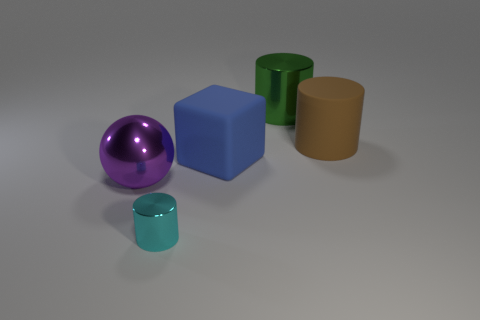
\includegraphics[scale=0.6]{figures/POVQAD中图像示例.png}
\caption{POVQAD中图像示例}
\label{POVQAD-figure}
\end{figure}
\item \textbf{$S_i$}为场景,是对当前图像中所有可见物体的ASP表示,采用ASP进行表示。
其中主要包含以下内容:每个可见物体的属性,包括尺寸、颜色、材质、形状;每个物体所属的区域;可见物体之间的空间关系,如\textbf{left(X,Y)}表示X在Y的左边;
被隐藏的物体(即问题中提及而图像中不存在的物体)不会出现在部分场景信息中。
\item \textbf{$Q_i$}为问题,使用自然语言形式进行表示,例如“What shape is the small red object that is to the left of the yellow cube?”。
所有问题均为属性查询类问题,专门针对物体的四个属性之一:颜色、尺寸、形状或材质。
\item \textbf{$QA_i$}为问题的ASP表示,例如:
\begin{lstlisting}
query(Q) :-
  has_property(X, color, Q),has_property(X, shape, cylinder),
  has_property(Y, shape, sphere),has_property(Y, color, red),
  left(Y, X),same_material(X, Y),X != Y.
\end{lstlisting}
\item \textbf{$\Pi_i$}为环境,是当前图像所属环境的一组约束规则,采用ASP进行表示。以下为一组约束示例:
\begin{lstlisting}
% 约束示例
% 区域0中所有物体的形状必须是圆柱体
:- obj(X), at(X, 0), has_property(X, shape, cylinder).
% 区域1中蓝色物体的数量大于2个
:- #count{X: has_property(X, color, blue), at(X, 1)} > 2.
\end{lstlisting}
\item \textbf{$A_i$}为答案集,表示该问题对应的正确答案。
\end{enumerate}
\section{构建流程}
POVQAD的构建流程如图\ref{fig:dataset-generation}所示,共包括5个步骤。各个步骤的功能如下:
\begin{enumerate}[nosep]
\item \textbf{生成环境}:随机选取部分约束模板,并将模板实例化,最终得到环境。
\item \textbf{构建场景图}:将环境实例化,并将环境输入ASP求解器进行求解,分别生成部分可见场景图和不可见场景图。
\item \textbf{图像渲染}:使用Blender对场景图进行渲染,获得积木世界图像与场景。
\item \textbf{问题生成}:根据问题模板与场景生成问题与其对应ASP查询,并使用Clingo得到问题的解,此外对答案集进行筛选。
\end{enumerate}
\begin{figure}[h]
\centering
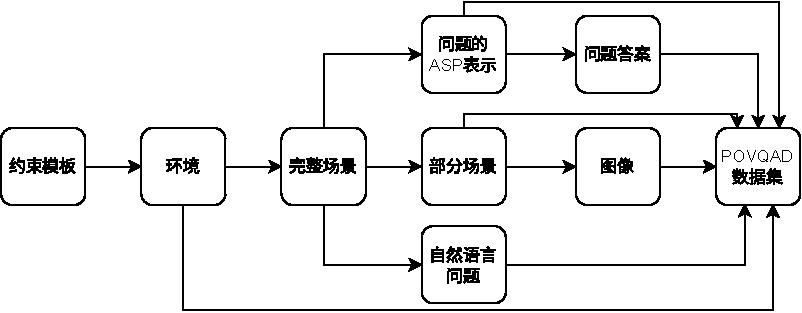
\includegraphics{figures/pipeline-POVQAD.drawio-crop.pdf}
\caption{POVQAD构建流程}
\label{fig:dataset-generation}
\end{figure}

\subsection{生成环境}
在POVQAD中,一个环境包含了一组约束规则,用于限定在该环境下生成的所有场景所必须满足的
属性组合、区域位置的约束条件。环境的作用是,在宏观层面上对后续生成的图像、问题进行把控,
以控制场景复杂度,并保证数据集保持逻辑一致性。在数学上可以如下表示环境:
$$ \varepsilon = \{C_1,C_2, ..., C_k \}, C_i \in ASP \quad Constraint $$
其中,每个$C_i$是用 ASP 表示的一条逻辑约束规则。

环境的生成过程包括以下步骤:(1)预定义11种约束模板;(2)确定模板中的相关参数;(3)对所有生成的约束经语义检查与逻辑一致性验证。

约束模板是依据常见的逻辑组合来进行设计的,覆盖了取值限定、逻辑否、逻辑或等基本逻辑模式,
部分约束模板的ASP编码表示以及对应表示含义见表\ref{tab:asp_templates},全部约束模板见附录\ref{appendix:constraints}。
除了约束模板之外,还有全局约束。
全局约束是所有生成的环境都应遵循的约束,对整个积木世界进行了基本定义,例如“平面区域划分为4个,编号0、1、2、3。”就是通过全局约束定义的,
ASP形式为\texttt{region(0). region(1). region(2). region(3).}。
本文所用的所有全局约束在附录\ref{appendix:environment}同样予以了展示。
\begin{table}[h]
    \centering
    \renewcommand{\arraystretch}{1.0}
    \begin{tabular}{|p{2.8cm}|p{12.2cm}|}
        \hline
        \textbf{模板} & \textbf{描述} \\
        \hline
        \textbf{模板1(取值约束)} & 
        \texttt{:- obj(X), at(X, R), not has\_property(X, P1, V1).} \\ 
        & 解释: 对区域R中的所有物体,它们P1属性的取值均为V1。 \\ 
        & 具体实现: :- obj(X), at(X, 0), not has\_property(X, color, red). \\
        \hline
        \textbf{模板2(遮挡比例约束)} & 
        \texttt{:- occlusion\_rate(T, R), (R <= 0; R >= 1).} \\ 
        & 解释:物体T被遮挡的比例为R(0<R<=1),完全遮挡时R=1。 \\ 
        & 具体实现::- occlusion\_rate(T, 0.1). \\
        \hline
    \end{tabular}
    \caption{部分约束模板示例}
    \label{tab:asp_templates}
\end{table}

模板实例化生成环境的过程中,需要设定一些参数,具体包括:
\begin{enumerate}[nosep]
\item \textbf{规则模板数量}:每个环境实例化多少条规则模板,规定单个环境最多实例化15条。
\item \textbf{属性类型}:将模板中的属性类型占位符用实际生成的属性类型进行替换,例如 P1' 替换为 color,P2' 替换为 shape。
\item \textbf{属性值}:用随机生成的属性值替换,例如 V1' 替换为 red,V2' 替换为 sphere。
\item \textbf{区域范围}:规则作用在哪些区域。根据POVQAD的定义,区域编号为0、1、2、3。
如果是全局作用的模板,则需要将该条规则的作用区域设置为0、1、2、3。如果是作用在局部区域,仅需设置某个或某几个区域即可。
\item \textbf{数量参数}:恰有、至少、至多约束中要求的具体数量。
\end{enumerate}

模板实例化之后,再基于所得的模板实例,为每个区域生成区域内约束,并随机生成跨区域约束和强制否定约束。
强制否定约束用于限制某些属性或者属性做个不能出现在特定区域中,跨区域约束用于限制多个区域之间对象的关系或者属性分布,区域内约束
用于限制单个区域内对象的属性或者属性组合。
最终,得到具体的约束表达式如下所示:
\begin{lstlisting}
:- object(X), at(X, 0), not hasProperty(X, color, red).
:- object(X), at(X, 1), hasProperty(X, shape, cube).
:- #count{sameProperty(X1, X2, color): object(X1), object(X2), at(X1, 0), at(X2, 1)} < 2.
\end{lstlisting}

POVQAD规定每个环境最多由15条约束规则模板实例化构成,这一数值是经过多方面权衡确定的,目的主要在于以下几方面:
\begin{enumerate}[nosep]
\item 逻辑复杂度与可解性的平衡。如果某个环境中的约束规则过少,会导致后续生成的场景过于松散,
物体属性组合高度自由,推理空间过大,导致问题复杂度过大,难以进行有效推理。
如果约束规则过多,则会造成约束之间产生冲突,导致ASP求解器难以知道合法的解,影响求解效率,进而影响场景的生成。
\item 控制生成时间与可维护性。每条规则在 ASP 中都可能极大影响解空间,规则数上升将显著增加 ASP 求解时间。此外,
在大规模数据生成中,15 条以内的环境可以在数秒内稳定求解出场景,利于批量生成和调试。
\end{enumerate}

在生成环境的过程中,规定每个环境中至少包括区域级约束和跨区域约束,共计两种约束。做出这一规定的目的在于
增强环境的逻辑层次性与推理深度,具体原因如下:
\begin{enumerate}[nosep]
\item 支持多层次推理链的构造。区域级约束用于构建局部一致性,跨区域约束用于建模全局对比或协同关系。
同时使用这两类约束,可以使推理问题具有从局部到跨区域的空间层级,增加问题的空间深度。
\item 避免场景构造退化为简单的组合。如果只使用区域级约束,那么后续根据环境生成场景时,将会变成多个局部区域的简单组合,
缺乏各个区域之间的相互关联。添加跨区域约束之后,有助于生成具有全局一致性/相互限制/相互支撑的复杂场景。
\item 支撑部分可见场景下的间接推理。在部分场景中,若不可见物体在区域0中缺失,模型可以通过区域0的其它规则
或者区域0与区域1的对比或者联动规则来进行属性排除或依存判断。而如果采用单一的区域级约束,
那么对于区域0中的物体的问题,模型只能依赖于区域0的局部信息进行推理,缺乏全局视角,不利于考察模型的宏观层面推理能力。
\end{enumerate}

此后在生成环境时,将全局约束与获得的约束表达式进行拼接,形成完整ASP程序,并由Clingo对ASP程序进行求解。
如果Clingo的输出至少存在一个答案集,说明当前约束可满足,将所得结果(即环境)保存到ASP程序的\texttt{.lp}文件中。如果Clingo没有答案集,说明当前约束不满足,会
尝试使用其它的约束表达式进行求解,直到能够生成一个环境。

进行语义检查与逻辑一致性验证的具体方案是用ASP求解器(本文中采用Clingo)对生成的约束尝试进行求解,
如果Clingo没有提示错误信息,并且能够成功求解出至少一个合法的解集,则说明该环境的约束规则是逻辑一致的,并且
能够顺利通过语法检查。本步骤的主要目标是避免后续出现死循环、空解等问题。

最终,一共生成了30个环境,数据集中的所有场景均匀分布在这些不同的环境之中。
控制生成30个环境的原因是,这一数量的环境实际上可以供后续生成数百万个不同场景和问题,足够支撑进行大规模训练与严格测试。
环境的具体示例见附录\ref{appendix:environment}。
\subsection{构建场景}
\subsubsection{构建完整场景图}
在获得环境约束后,需要进一步获得符合约束的场景图,所需流程为:
将获得的环境约束Clingo进行求解,生成符合约束的答案集,并对答案集进行采样。一个答案集
对应一个完整场景图。此后,将答案集进行解析,获得完整场景图。

首先,将包含了环境约束的\texttt{.lp}文件提交至Clingo进行求解,对Clingo的输出结果进行简单解析,将所有答案集进行提取。

在生成答案集之后进行采样出于以下两点原因:
\begin{enumerate}[nosep]
\item 避免处理过多的答案集。如果直接处理所有答案集,会导致后续的场景生成和问题生成过程耗费大量时间和资源。
\item 控制场景的多样性。如果直接使用所有答案集,可能会生成大量相似的场景,导致数据集的多样性不足。
某些约束可能会导致生成的场景具有高度重复的物体属性或关系。随机采样可以增加场景的多样性,避免生成过于相似的场景。
\item 平衡约束类型的答案集。不同的约束类型可能会生成不同数量的答案集。
如果某些约束类型生成的答案集过多,而其他约束类型生成的答案集较少,可能会导致数据集中某些类型的场景占比过高。
对每种约束类型的答案集进行采样,可以平衡不同约束类型的场景数量,确保数据集的均衡性。
\item 降低后续处理的复杂度。每个答案集需要进一步解析为场景图,并用于生成图像和问题。
如果答案集数量过多,会显著增加后续处理的复杂度。通过减少答案集数量,降低后续处理的复杂度,确保生成管道的可控性。
\end{enumerate}

场景是最终渲染的图像及其对应的描述信息,包括图像中的所有物体及其属性和位置。场景以JSON文件存储,某个场景如下所示:
\begin{lstlisting}

\end{lstlisting}

场景图是场景的结构化表示,描述了场景中物体的属性以及物体之间的关系,是场景的一种中间表示。某个场景图如下所示:
\begin{lstlisting}
{
  0: {"color": "red", "shape": "sphere", "size": "large", "material": "rubber", "region": 0},
  1: {"color": "blue", "shape": "cube", "size": "small", "material": "metal", "region": 1}
}
\end{lstlisting}

对答案集进行解析的过程实际上是对谓词进行解析的过程,会将\texttt{has\_property}和\texttt{at}两个谓词进行解析,
最终形成以JSON格式存储的场景图。

此后基于所得的完整场景可以生成部分可见场景和不可见场景。以下两小节将展开介绍。
\subsubsection{构建部分可见场景图}
部分可见场景与完整场景的区别在于:部分可见场景中增加了对于物体之间遮挡关系以及遮挡比例的规则,进而后续Blender根据场景
渲染图像时,能够得到场景中描述的部分物体之间存在遮挡的图像。构建部分可见场景的具体流程如下:

首先从完整场景中,随机选取两个物体,并分别指定一个物体为将会被提问的目标物体\texttt{T}
,另一个物体为去遮挡目标物体的\texttt{Oc}。
此后,向场景中添加ASP谓词\texttt{target(T)}、\texttt{occluder(Oc)}以及\texttt{occludes(Oc,T)},分别表示
\texttt{T}为目标物体,\texttt{Oc}为遮挡物体,Oc在图像中遮挡了T。此后,生成一个介于0和1之间的随机数$R$,用于表示目标物体
被遮挡的面积比例。本文规定$R$大于0且小于1。当$R=1$时,相当于目标物体被完全遮挡,对应不可见场景的构建,为其它不同的构造方法。

此后,再随机选择目标物体\texttt{T}的形状、颜色、材质、尺寸中的任意一个属性,将其从场景中移除,以表示由于该物体被遮挡导致的信息缺失。
\subsubsection{构建不可见场景图}
基于完整场景构图建不可见场景图的构造思路是:从完整场景图中随机移除一个对象。

本环节的目标是,从完整场景中随机选择一个物体作为被隐藏的目标物体,并围绕该物体构造相关问题
,并同时使用自然语言及ASP对问题进行表示。
整个环节的流程图如\ref{generate-partial-scenes-and-questions}所示。
\begin{figure}[h]
\centering
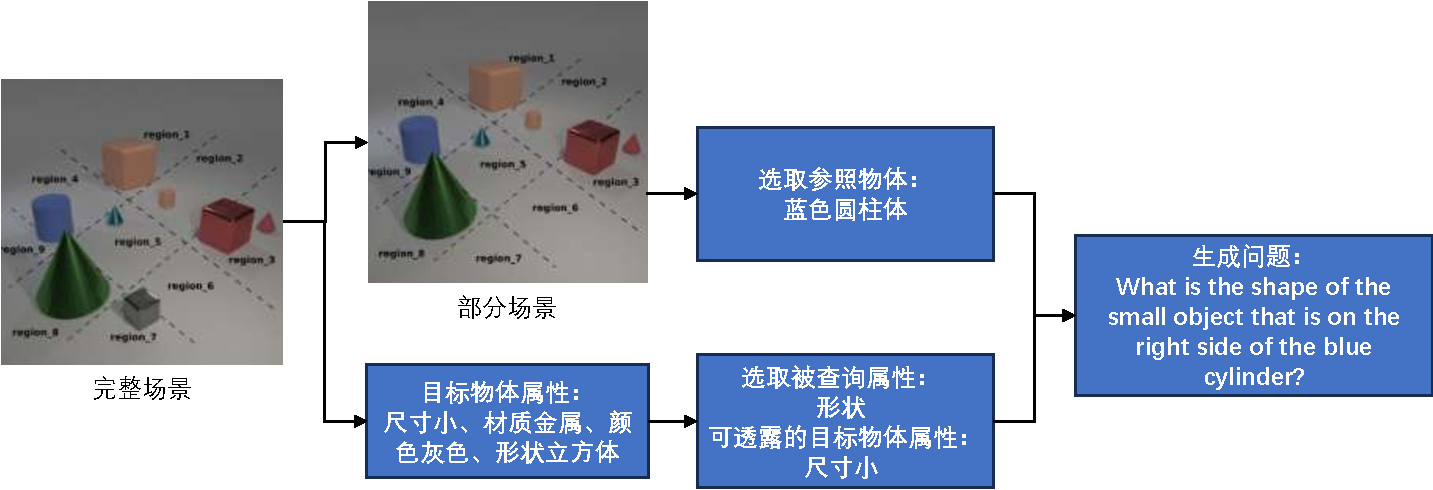
\includegraphics[scale=0.6]{figures/部分场景及问题生成-crop.pdf}
\caption{构建部分场景并生成问题流程图}
\label{generate-partial-scenes-and-questions}
\end{figure}

选择目标物体的过程需要满足以下条件:
\begin{enumerate}[nosep]
\item 从完整场景的所有物体中随机选取一个,在随机选取的过程中,要注意保持均衡,不能
一直选取单一区域的物体或者相同属性的物体,以免造成数据偏态分布。
\item 被选择物体不能是唯一出现某一属性的对象,避免由于移除该物体后,
导致场景中该属性的值无法被推断,导致问题无解。
\item 该物体将在后续问题中作为查询目标。
\end{enumerate}

选择$Obj_i$后,需要将完整场景中关于$Obj_i$的所有事实全部移除,生成部分场景。具体需要做到以下几点:
\begin{enumerate}[nosep]
\item 删除\texttt{obj(i)}、\texttt{at(i, R)}、\texttt{has\_property(i, P, V)};
\item 删除所有涉及$Obj_i$的空间关系谓词,如\texttt{left(i, j)}、\texttt{right(i, j)}等;
\item 保留其余物体的信息与关系。
\end{enumerate}
从而得到一个只包含可见物体的子结构,记为 $Partial_i$,该场景中缺少了目标物体的显式信息。

随后,将根据$Obj_i$的属性来生成相关问题。
每一个生成的问题,应该满足如下条件:(1)针对被隐藏对象的某一属性;
(2)基于剩余可见物体和环境约束进行间接推理;(3)问题语义必须明确且答案集非空。
以某个问题的生成为例,$Obj_i$的属性包括:尺寸为小、材质为金属、颜色为灰色、形状为立方体
,那么可以随机选取形状作为被查询属性,并将“尺寸为小”作为已知信息放置在问题当中。
为了便于控制问题类型的数量分布,本文规定每个问题只能查询上述四个属性中的一个,而不同时查询多个属性。
与此同时,问题生成器也将从图中选取一个
参照物体,用以共同组成问题。考虑到不同种类属性的可能取值数量不同,进而不同属性的问题的可能答案数量也不同,
本文据此规定每种属性的问题在数据集中所占的比例:颜色与形状各占40\%,材质与尺寸各占10\%。
该比例同样通过ASP约束来进行实现。
需要注意生成的问题仅为属性查询问题,不包括是非题和计数题等其它CLEVR中原有的问题类型,理由在3.1节构建目标中已有陈述,此处不再赘述。

\subsection{图像渲染}
图像渲染与样例生成的目的是将部分可见场景图以及不可见场景图转换为场景,并使用Blender进行渲染。

\begin{enumerate}[nosep]
\item 初始化Blender渲染对象。在这一步中,主要是设置一系列渲染参数,包括分辨率、GPU设置等等。
\item 定义场景字典。该字典中保存了场景的元信息(即将生成的图片名称等)、物体信息和方向信息。
\item 方向向量计算。先获取在场景初始化时添加的平面的法向量,此后计算摄像机的方向向量,并将
摄像机的方向向量投影到平面上,得到相对于平面的方向向量。计算完成之后,将平面删除,避免影响后续渲染
\item 向场景中添加物体。根据场景图中的物体信息,将物体添加到场景中。添加过程中,要注意确保物体之间的距离和边距满足约束条件。
此外,在生成部分可见场景时,要注意根据部分可见场景图中的遮挡物体和遮挡面积比例,来生成遮挡的情形;
在生成不可见场景时,要注意。
\item 计算物体之间关系。基于物体的三维坐标和场景的方向向量,遍历场景中的每对物体,
计算得出空间中上、下、左、右、前、后等关系。判断两个物体之间是否存在某种关系的阈值设置为0.2,即如果两个物体之间的
方向向量的点积大于0.2,那么认为它们具有该关系。

最终,输出一个JSON对象,其中描述了场景中所有物体之间的空间关系,一个可能的字典如图所示,其中$left[0] = 1$说明
物体0的左侧有物体1,$right[1] = 0$说明物体1的右侧有物体0。
\begin{lstlisting}
{
    "left": [[1], [], [], []],
    "right": [[], [0], [], []],
    "above": [[], [], [3], []],
    "below": [[], [], [], [2]],
    "front": [[], [], [], []],
    "behind": [[], [], [], []]
}
\end{lstlisting}
\end{enumerate}

在图像渲染完成之后,整个场景构造完成,此时进行数据整合,将所有场景文件合并同一个包含所有场景的JSON文件中。

\subsection{问题生成}
POVQAD根据前述步骤整合的场景文件和问题模板来构造自然语言问题,
一种供参考的模板如\ref{asp:question-template}中所示,
其中<Z2>、<C2>、<M2> 表示待查询对象的已知属性(例如尺寸、颜色、材质),由随机策略从完整场景中选取;
<R> 为空间关系(如left、right、front、behind),其取值既满足随机性,又依赖于完整场景中物体间的真实空间分布;
<Z>、<C>、<M>、<S> 则代表参考对象的属性。这种模板化设计不仅使自然语言问题的结构化描述成为可能,
而且便于后续转换为ASP的形式化表示,从而实现问题求解的自动化。
\begin{lstlisting}[label=asp:question-template]
What shape is the < Z2 > (size) < C2 > (color) < M2 > (material) [that is] 
< R > (relation) the < Z > (size) < C > (color) < M > (material) < S > (shape) ?
\end{lstlisting}

首先,筛选问题模板。对模板的筛选,按照模板的查询目标是否与当前场景相匹配,以及模板中给定信息是否在场景中存在来进行。例如,对于下列问题模板,其提问的是
“物体A是否在物体B的上方?”但是该场景图中,两物体之间的
\begin{lstlisting}

\end{lstlisting}

问题模板筛选完毕之后,根据场景图和筛选好的问题模板,进行模板实例化,生成问题文本及其对应的ASP查询。
实例化过程中,需要对模板中的占位符替换为具体的属性值。对每一个自然语言问题,都是从一个问题模板出发,填充占位符,
然后生成的。所以,自然语言和ASP查询具有一一对应的逻辑结构,可以实现自动转换。

此后调用Clingo求解查询,生成问题的答案,并通过对答案进行分析,实现对生成问题的筛选。
筛选逻辑是:如果答案集为空或者包含所有的可能值,则丢弃当前问题。对生成问题进行筛选有以下三点原因:
\begin{enumerate}[nosep]
\item 提高问题的质量。确保生成的问题有明确的答案,而不是模糊或无意义的问题。
\item 避免冗余问题。避免生成答案集过大的问题,这些问题可能对模型训练没有帮助。
\item 确保问题的多样性。筛选掉覆盖所有可能答案的情况,确保问题具有一定的区分性。
\end{enumerate}

最后,将生成的问题、ASP查询和答案保存为JSON文件,以下为一个示例:
\begin{lstlisting}
{
    'split': scene_info['split'],
    'image_filename': scene_fn,
    'image_index': image_index,
    'question': ts,
    'program': qs,
    'asp_query': asp_query,
    'answer': possible_sols,
    'object_interest': obj_interest,
    'template_filename': fn,
    'question_family_index': idx,
    'question_index': image_index
}
\end{lstlisting}

\section{数据集质量评估}
为验证构造的POVQAD数据集的可靠性与研究价值,本节从POVQAD的可执行性与一致性、统计分析、对比实验方面进行研究。
\subsection{可执行性与一致性评估}
可执行性指的是POVQAD中每个样例的ASP程序能够经Clingo求解器执行,不出现语法错误。
一致性指的是对POVQAD中每个样例的ASP程序,Clingo对其的求解结果与样例中给出的标准答案一致。

本文对POVQAD中所有ASP程序依次使用Clingo进行执行,统计语法错误率,结果为0.2\%,
并且对能够正确执行的ASP程序的运行结果与标准答案进行对比分析,一致率为99.5\%,以上两点证明本文生成的ASP程序质量较高,
使用ASP构造POVQAD的方法合理。
\subsection{统计分析}
POVQAD中问题分布的统计图见图\ref{fig:question_statistics}。从图\ref{fig:question_statistics}(a)中可得知,有关颜色和形状的问题在POVQAD数据集中
占比最高,分别是39\%和37.6\%,关于大小和材质的问题则相对较少,分别只占到了13.6\%和9.8\%。
所提问题的类型取决于被查询的物体的属性,在生成数据集的过程中,允许用户设置问题类型的预期占比。
以上统计得到的POVQAD中问题类型占比,是基于以下的设置生成的:颜色问题占比40\%,形状问题占比40\%,大小问题占比10\%,材质问题占比10\%。
做出如上设置的原因是,与材质(只有两个值)相比,颜色和形状等属性包含更大的值集合(颜色有 8 个值,形状有 4 个值),
则对颜色和形状提问的问题有更多的潜在答案,故应将颜色和形状的相关问题的占比调高,以充分展示相关问题的答案集空间。

图\ref{fig:question_statistics}(b)、(c)、(d)和(e)分别说明了各种问题类型(尺寸、形状、材质和颜色)的潜在答案的分布。
生成数据集的目标之一是实现均衡的分布,避免大多数问题都导致相同的答案集的情况。
例如,当问题涉及物体的大小时,其可能的解可以是
 \{大, 中\}、\{大, 小\}、\{小, 中\}、\{大\}、\{中\} 或 \{小\} 之一,
 如图\ref{fig:question_statistics}(b)所示。由于查询属性为颜色的问题的可能答案数量很大(因为颜色可以取 8 个值),
 因此图\ref{fig:question_statistics}(e)中并未列出整个空间。根据统计图可以看出,在生成过程中没有偏向任何特定的答案。
\begin{figure}[h]
    \centering
    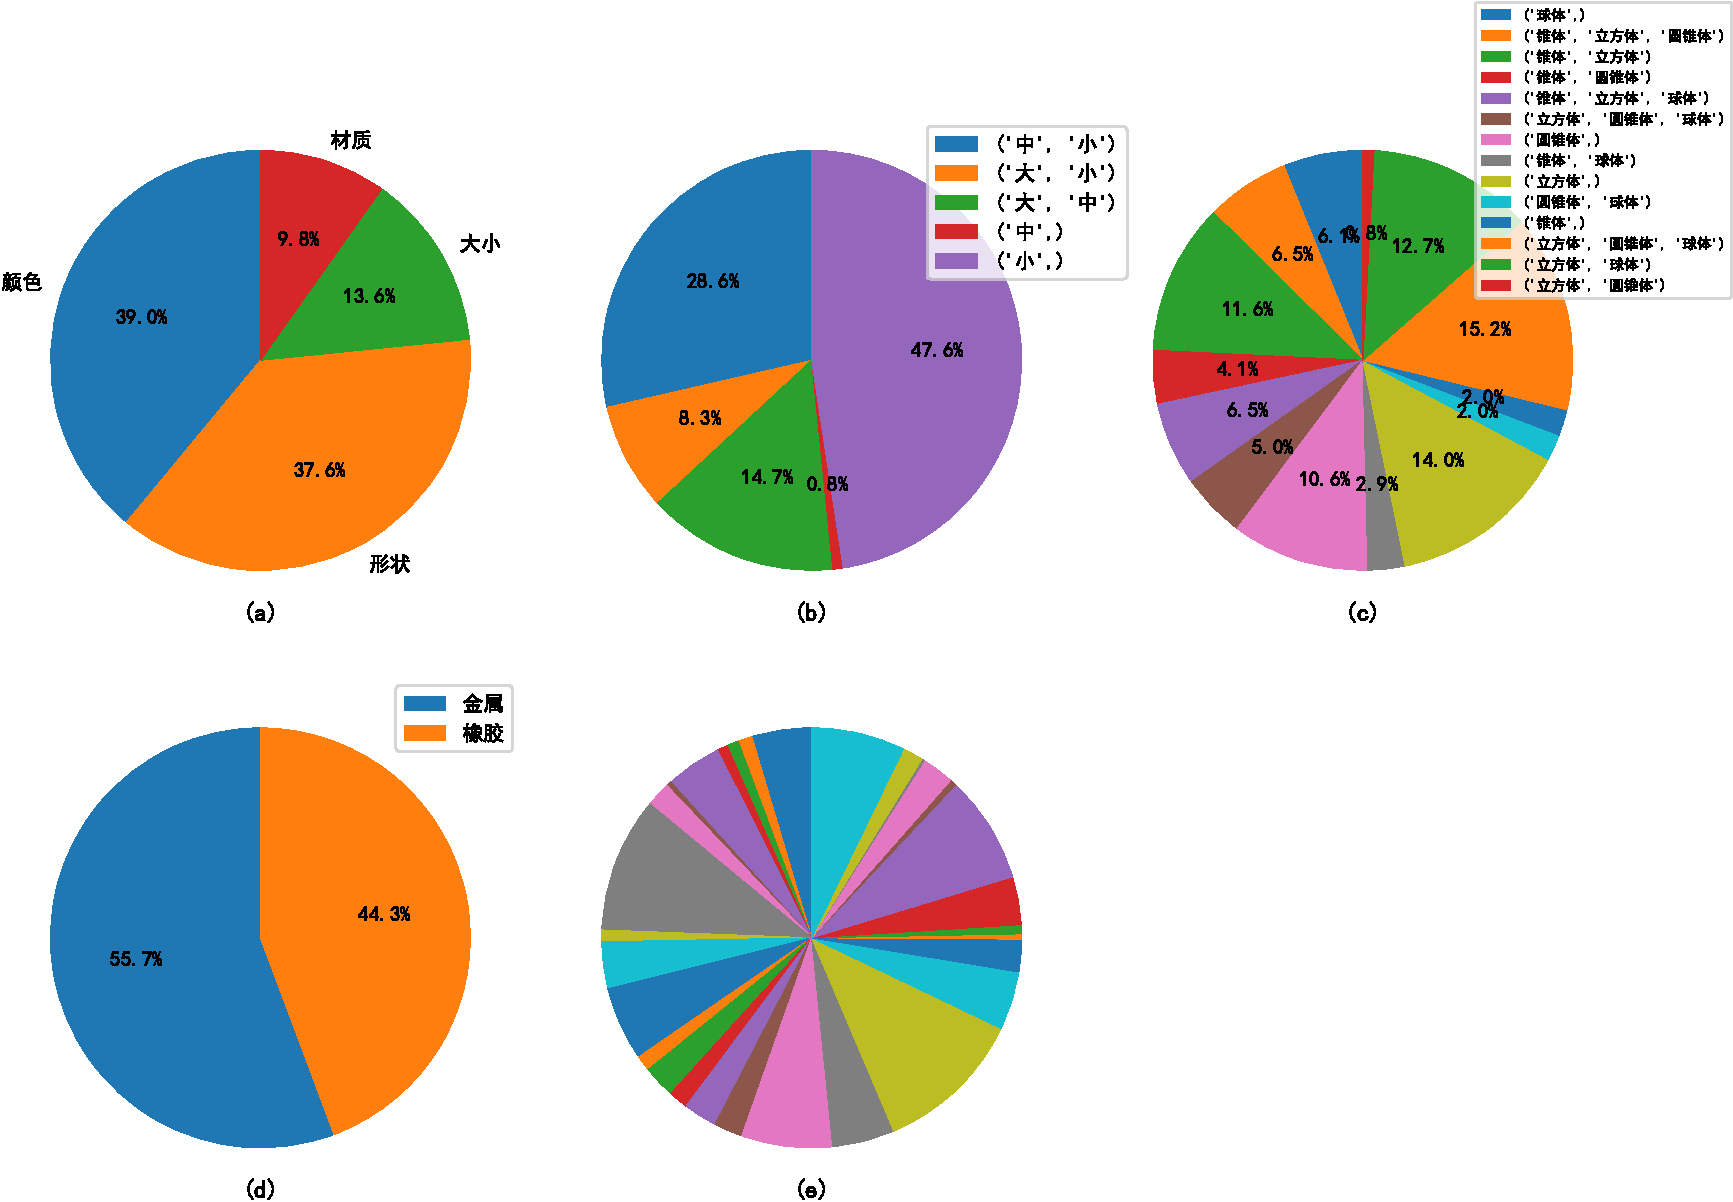
\includegraphics[scale=0.45]{figures/question_distribution-crop.pdf}
    \caption{问题分布统计}
    \label{fig:question_statistics}
\end{figure}

图\ref{fig:template_statistics}(a)中展示了POVQAD中问题在不同问题模板上的分布情况,\ref{fig:template_statistics}(b)中展示
了特定类型问题根据场景中物体数量划分的分布情况。
\begin{figure}[h]
    \centering
    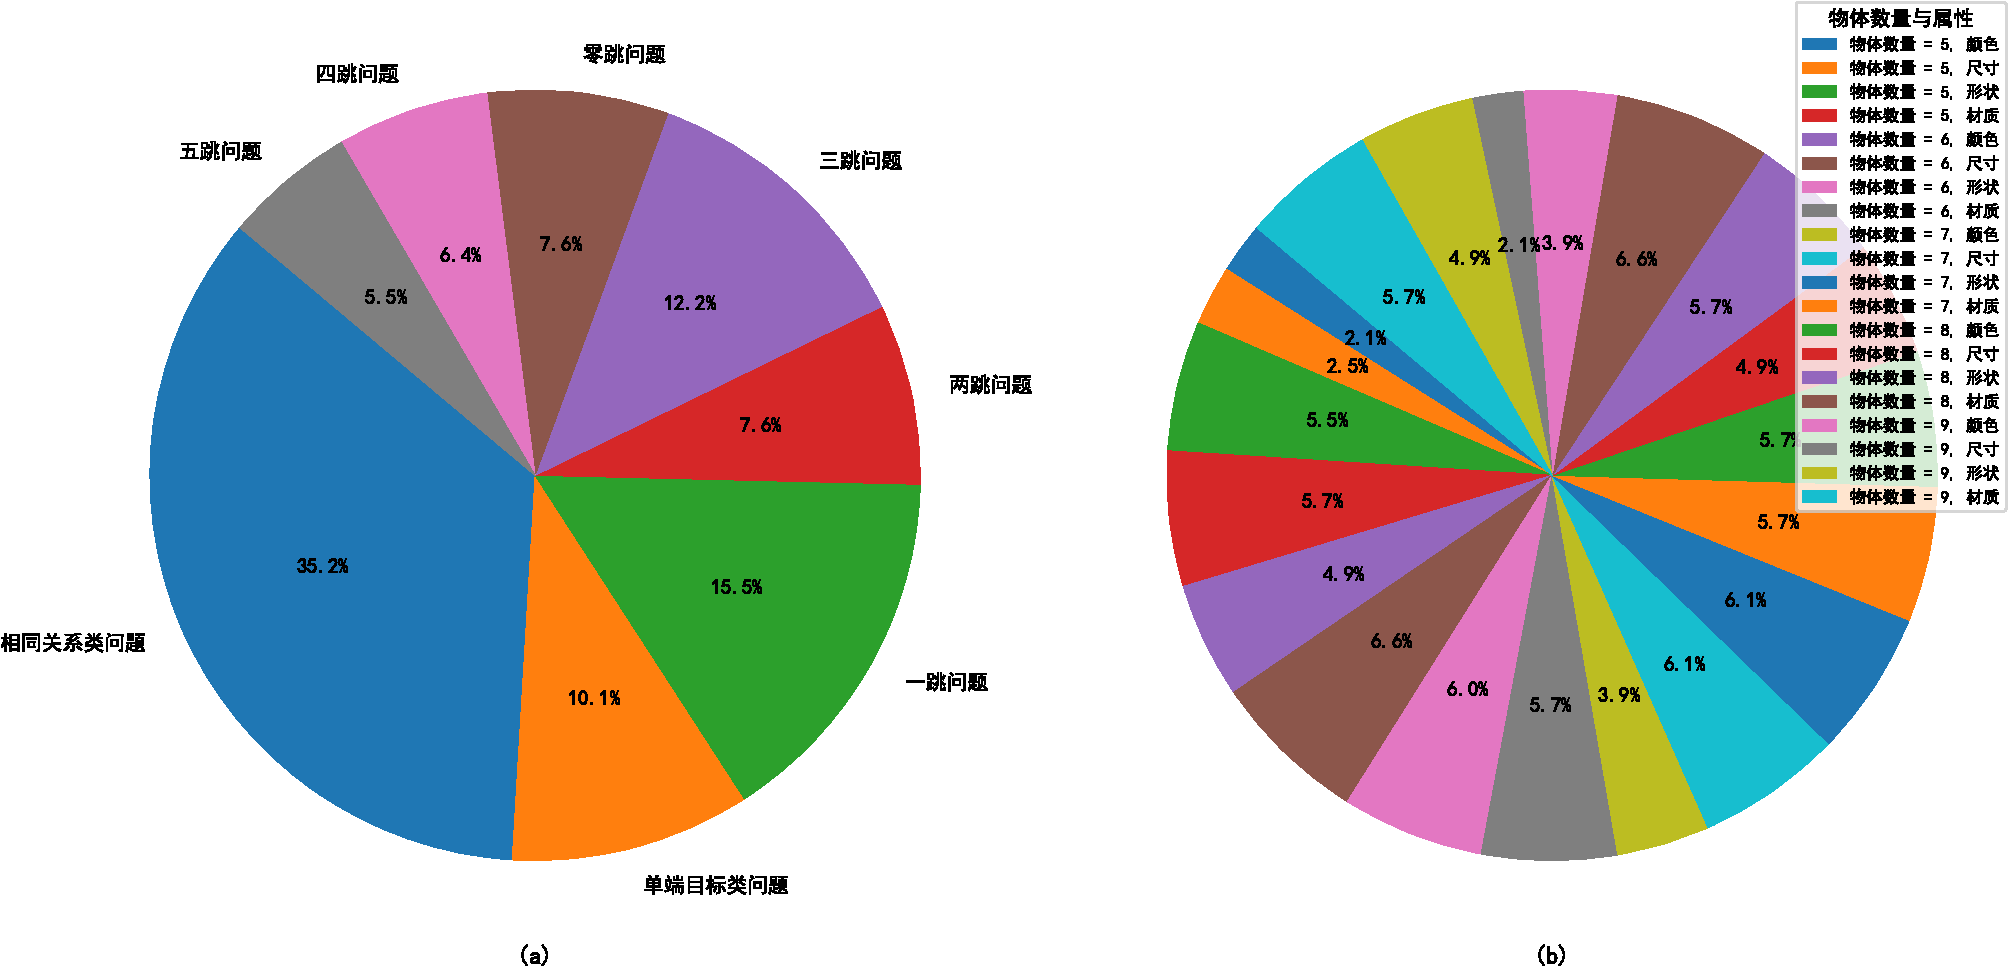
\includegraphics[scale=0.45]{figures/question_template_distribution-crop.pdf}
    \caption{问题模板分布情况}
    \label{fig:template_statistics}
\end{figure}
\subsection{对比实验}
为了证明POVQAD数据集对不同推理能力方法的区分性与挑战性,
本文选取了五种代表性方法在该数据集上进行实验:传统感知模型(CNN+LSTM)、
主流多模态大模型(DeepSeek、Gemini 2.5 Flash、ChatGPT-4o),以及人类作答作为理论上限参考。
每种方法的输入为POVQAD的图像、自然语言问题以及环境约束。实验重复进行三次取平均值,最终实验结果如图\ref{fig:dataset-comparison}所示,可得出如下结论:
\begin{enumerate}[nosep]
\item 数据集具有良好的难度区分能力。各方法在POVQAD上的准确率差异明显,充分体现了模型间的空间理解与逻辑推理能力差距。尤其是传统模型(CNN+LSTM)仅达到 45.4\% 的准确率,明显低于VLMs方法,显示POVQAD对浅层感知模型构成了挑战。
\item 多模态大模型在不完全信息推理方面存在性能瓶颈。
即便是先进的多模态大模型(如 ChatGPT-4o)也未能达到人类水平,
在复杂场景、信息遮挡和规则约束下的准确率仍有明显提升空间,说明POVQAD能有效考察模型对隐含信息与环境规则的建模能力。
\item POVQAD能作为更强推理任务的评估基准。
结果表明,POVQAD能有效区分浅层感知模型与具备显式推理机制的方法,
同时能检测当前主流多模态模型在空间推理与知识补全方面的能力边界,具备良好的基准测试价值。
\end{enumerate}
\begin{figure}[h]
\centering
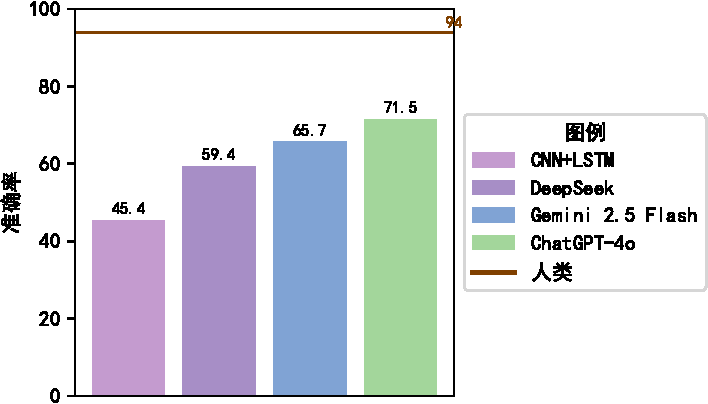
\includegraphics[scale=0.8]{figures/dataset-experiment-crop.pdf}
\caption{不同方法在POVQAD上回答问题的准确率}
\label{fig:dataset-comparison}
\end{figure}
\section{本章小结}
本章聚焦CLEVR数据集的场景完全可见、不要求模型使用外部背景知识进行推理等方面的缺陷,构建一个新的数据集POVQAD,以满足
本文对部分可见积木世界场景下空间推理问答的研究需要。

本章为后续神经符号VQA框架在部分可见积木世界场景下的空间推理问答的实验与分析奠定了坚实的数据基础。

\chapter{实验及结果分析}
\section{实验设计}
\section{结果分析}
\section{本章小结}

\chapter{问答系统的构建}
\section{需求分析}
本系统旨在基于本文提出的神经符号框架,构建一个视觉问答系统,既能利用深度学习技术对图像进行特征提取,用LLM对自然语言进行语义解析,又能通过ASP
求解器实现推理,同时为用户提供友好、直观的前端交互界面。

\subsection{功能需求}
核心功能上,需要实现以下几个功能:(1)用户输入与对话处理。系统需要能够支持文本输入、图像输入,未来远期可以考虑加入语音输入。此外,提供自动补全、拼写检查等输入辅助功能,
以改善用户的输入体验。(2)实时对话回复。系统能够通过Dspy的SDK,发起对本地LLM的调用,而LLM能够实时处理用户的问题,返回高质量的回答。另外,要能够支持多轮对话,
能够保持上下文关联,具有记忆功能。(3)对话历史记录。系统需要能够自动保存用户每次的对话记录,以供用户查看。(4)帐户与认证。系统需要支持用户注册、登录
、账号设置等功能。(5)数据统计与反馈。系统需要收集交互数据(如访问量、对话时长、常见问题等),供后续模型优化使用。另外,要提供用户反馈入口,支持用户评价回复质量。

辅助功能方面,主要围绕以下几点:(1)响应式设计。前端能够自适应桌面、平板和手机等不同设备。(2)辅助说明。提供FAQ、帮助文档
和使用指南,方便用户进行查阅。(3)安全与异常处理。能够对恶意输入、不符合规范的输入进行拦截和提示。
\subsection{非功能需求}
非功能需求主要聚焦于以下几个方面:(1)性能需求。系统需要能够在较短时间内完成对用户问题的回答,如果确实因为某些原因导致无法及时回答,需要能够给出合理的提示,
例如“正在思考...”等。另外,各个微服务应支持高并发访问,保证系统能够承受一定规模的大流量访问。(2)可拓展性。对系统要按照主要功能来进行拆分,形成若干个微服务,
并且各个微服务之间要能够相互独立,实现松耦合。当系统需要进行拓展时,只需要增加新的微服务,而不需要对原有的微服务进行修改。(3)可维护性。代码和文档需要保持清晰,
易于理解和修改,特别是对于接口文档,要使用Swagger等工具进行规范化管理,以便于后续的维护和拓展。另外,要提供清晰的日志记录、监控报警机制,使用一些监控
工具,如Prometheus、Grafana等,对系统的运行状态进行监控,及时发现问题并解决。(4)安全性。用户的数据传输和存储需要进行加密,对于用户的隐私数据,例如
手机号、密码等,需要进行脱敏处理,以保证用户的隐私安全。此外,对登录、注册等操作,需要进行身份验证和权限控制,防止恶意攻击。(5)可用性和用户体验。
在整体外观上,系统需要提供简洁友好的用户图形界面,降低使用门槛。

\section{架构设计}
\subsection{总体架构}
对本系统的总体架构设计如图\ref{fig:overall_architecture}所示。

后端部分采用微服务架构设计,包括视觉场景理解服务、语义解析服务、符号推理服务、迭代反馈服务、答案生成服务、
用户交互服务、日志与监控服务、数据存储服务等。各微服务之间通过API网关进行通信,API网关负责请求的路由、负载均衡、安全认证、限流等功能。

具体到各个
微服务的主要职能如下:(1)视觉场景理解服务负责对用户上传的图片进行目标检测,并使用预定义的谓词,使用ASP程序来表示场景中的物体的相关信息;(2)
语义解析服务负责将用户的自然语言问题转化为ASP规则,以便于后续的推理;(3)符号推理服务负责对ASP规则进行推理,得到问题的答案;(4)迭代反馈服务
负责对ASP规则进行修正;(5)答案生成服务负责将符号推理服务输出的以ASP谓词表示的答案转化成自然语言;(6)用户交互服务负责提供用户接口,
接收用户的输入,调用其他服务,返回结果;(7)日志与监控服务负责记录系统的运行日志,监控系统的运行状态,及时发现问题并解决;(8)数据存储服务负责
存储系统的数据,包括用户的信息、对话记录、ASP规则等。

前端部分,对UI界面的开发,选择Element UI框架,其具有丰富多样的按钮、输入框等搭建网页所需的元素,开发快捷方便。同时,使用Axios
向后端发送请求,实现前后端的数据交互。使用Vue构建组件化的前端页面,方便代码的维护和拓展。Vue Router用于实现前端路由,实现页面的跳转。Vuex用于实现状态管理,方便组件之间的数据传递。

在中间件上,系统引入了Sentinel进行流量控制,对系统的流量进行监控,实现限流、熔断等功能。RocketMQ用于实现消息队列,实现微服务之间的异步通信。
Redisson用于实现分布式锁,保证系统的并发安全。
\begin{figure}[htbp]
    \centering
    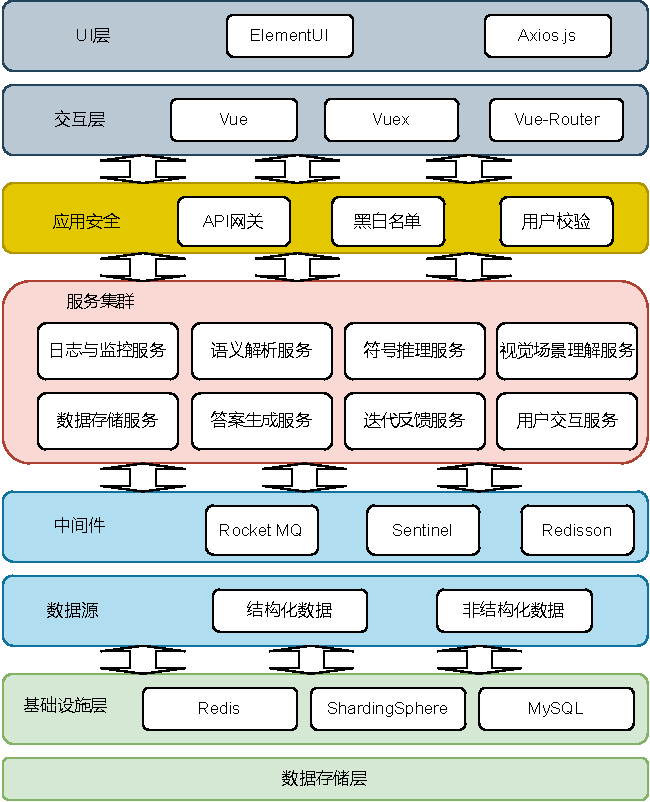
\includegraphics{figures/system_architecture-crop.pdf}
    \caption{系统总体架构}
    \label{fig:overall_architecture}
\end{figure}
\subsection{接口设计}
接口设计总体按照服务划分,每个服务提供一个接口供其它服务调用。接口之间的数据传输采用JSON格式,采用RESTful API设计风格。
具体的接口设计方案见表\ref{}。
\

\subsection{安全设计}
安全设计主要聚焦数据存储加密、用户认证。

\subsection{数据库设计}
设置User、Rule、Log、Dialog以上四个数据库。下面,对这四个数据库的职责及内设表进行介绍。

User数据库主要用于存储用户、角色、权限、会话信息等。内部包含如下表:(1)用户表users,用于存储用户信息 ;
(2)用户组表roles,用于存储用户组信息;(3)用户组关系表user\_roles用于存储用户与用户组之间关系;(4)用户状态表user\_session,用于存储会话或者登录状态记录。

Rule数据库专门用于存储ASP规则及其相关信息。内部包含rules表和rule\_conditions表。rules表为主规则表,rule\_conditions表为规则条件表。具体表字段见
表\ref{tab:rule}。
\begin{table}[htbp]
    \centering
    \renewcommand{\arraystretch}{1.3} % 调整行间距
    \resizebox{\textwidth}{!}{
    \begin{tabular}{|l|l|l|}
        \hline
        \textbf{字段名称} & \textbf{数据类型} & \textbf{说明} \\ 
        \hline
        rule\_id & INT AUTO\_INCREMENT PRIMARY KEY & 规则唯一标识 \\ 
        \hline
        rule\_name & VARCHAR(255) & 规则名称 \\ 
        \hline
        rule\_head & VARCHAR(255) & 规则若论部分 \\ 
        \hline
        priority & INT & 优先级 \\ 
        \hline
        status & ENUM('active', 'inactive') & 状态标识 \\ 
        \hline
        description & TEXT & 描述或备注 \\ 
        \hline
        created\_at & DATETIME DEFAULT CURRENT\_TIMESTAMP & 创建时间 \\ 
        \hline
        updated\_at & DATETIME DEFAULT CURRENT\_TIMESTAMP ON UPDATE CURRENT\_TIMESTAMP & 更新时间 \\ 
        \hline
    \end{tabular}
    }
    \caption{rule表字段设置及说明}
    \label{tab:rule}
\end{table}
\begin{table}[htbp]
    \centering
    \renewcommand{\arraystretch}{1.3} % 调整行间距
    \resizebox{\textwidth}{!}{
    \begin{tabular}{|l|l|l|}
        \hline
        \textbf{字段名称} & \textbf{数据类型} & \textbf{说明} \\ 
        \hline
        condition\_id & INT AUTO\_INCREMENT PRIMARY KEY & 条件唯一标识 \\ 
        \hline
        rule\_id & INT & 外键,关联到主规则表 \\ 
        \hline
        condition\_text & VARCHAR(255) & 单个条件表达式,例如"X > 10" \\ 
        \hline
        sequence & INT & 条件顺序号,用于保持条件排列 \\ 
        \hline
        created\_at & DATETIME DEFAULT CURRENT\_TIMESTAMP & 创建时间 \\ 
        \hline
        updated\_at & DATETIME DEFAULT CURRENT\_TIMESTAMP ON UPDATE CURRENT\_TIMESTAMP & 更新时间 \\ 
        \hline
    \end{tabular}
    }
    \caption{rule\_condition表字段设置及说明}
    \label{tab:rule_conditions}
\end{table}

Log数据库存储系统运行日志、错误日志、操作记录等信息。其内部包含如下表:(1)系统日志表system\_logs,用于记录系统一般日志;(2)错误日志表error\_logs,用于记录错误信息;
(3)审计日志表audit\_logs,用于记录关键操作审计日志。

Dialog数据库存储所有用户与系统的对话记录。其内部包含如下表:(1)对话主表dialogs,用于记录每个对话的基本信息;(2)对话消息表dialog\_messages,用于
存储对话中用户发出的消息与LLM给出的每条回复。

\section{功能展示}
开发的前端页面如图\ref{fig:welcome-page}所示,采用了模仿ChatGPT的网页样式。
用户可在其中自行选择模型,包括本文中微调后的模型、OpenAI的GPT系列模型、Google的Gemini系列模型、Meta的Llama系列模型
以及阿里巴巴的QWen系列模型,默认选用本文的微调后模型。用户可以在下方的菜单栏中,点击第二个按钮,以上传图片。同时,历史对话也会在左侧栏中予以显示。在
输入框旁,也添加了语音输入按钮,点击后系统将会调用百度的语音识别API,为用户提供语音输入服务。

上传图片并提出问题、系统给予答复后的效果如图\ref{fig:question}所示。用户发送的文本和图片将会在同一个消息框内显示。用户要求系统重新生成回复,或者引用系统的某条回复,以让系统能够更加贴合用户的语境。

\begin{figure}[htbp]
    \centering
    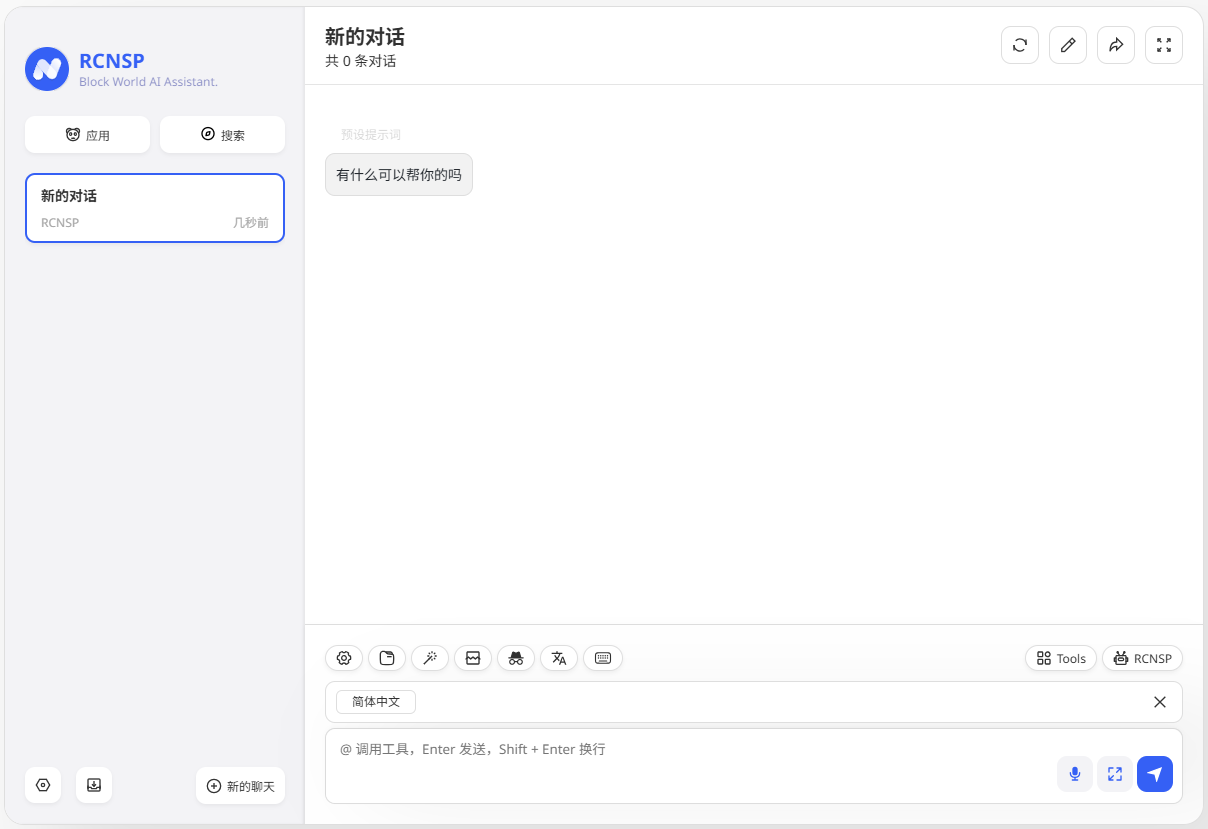
\includegraphics[width=\textwidth]{figures/frontend-welcome-page.png}
    \caption{新对话页面}
    \label{fig:welcome-page}
\end{figure}
\begin{figure}[htbp]
    \centering
    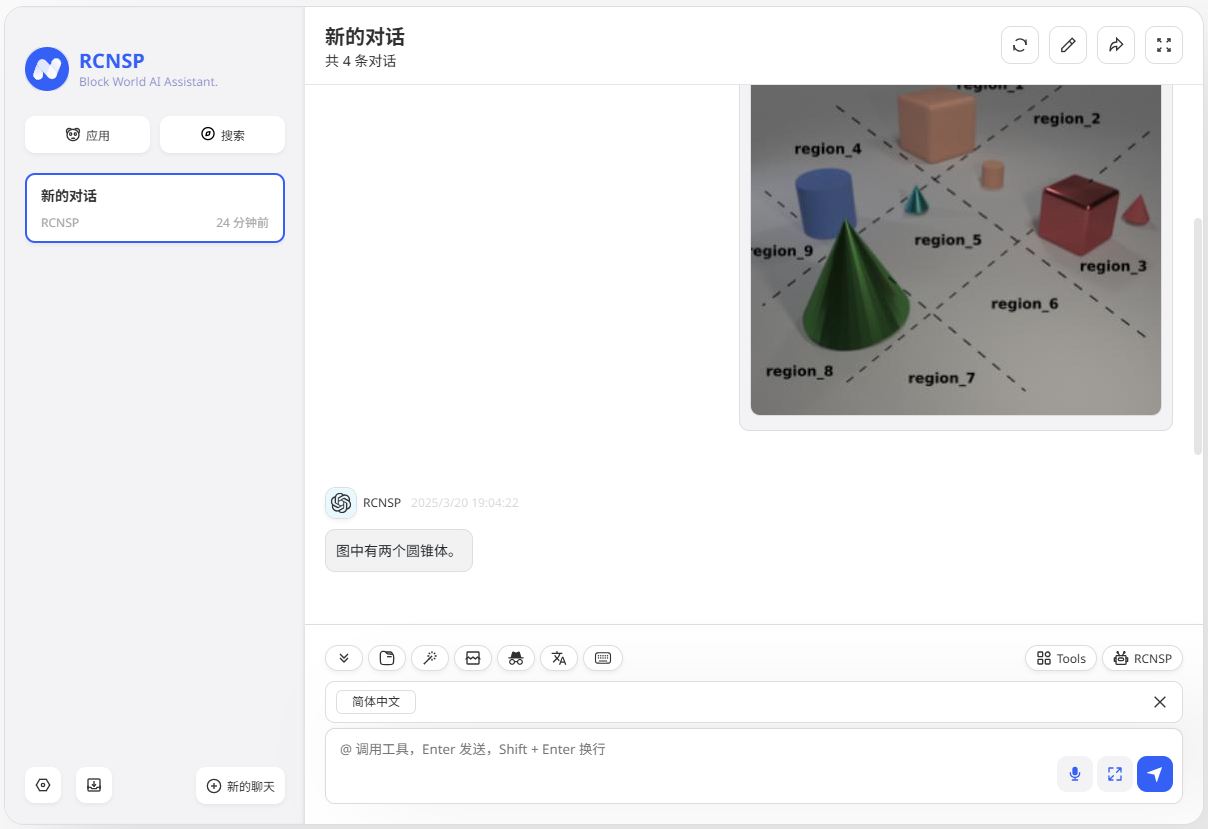
\includegraphics[width=\textwidth]{figures/question.png}
    \caption{上传图片并提问后的效果}
    \label{fig:question}
\end{figure}


\section{集成测试}
\subsection{测试环境}
系统的部署运行环境的硬件配置如下:(1)CPU为Intel Core i9-13900K;(2)内存为128GB;(3)显卡为3张NVIDIA GeForce RTX 3090并联,显存均为24GB;(4)操作系统为Ubuntu 20.04 LTS;
开发工具为IntelliJ IDEA、IntelliJ Pycharm和Microsoft Visual Studio Code。
\subsection{功能测试}

\subsection{非功能测试}
非功能性需求中,需要通过测试以量化评估的主要为性能需求。因此,本文通过压力测试,对系统的性能进行评估。
本文使用JMeter工具进行压力测试。JMeter是一种开源的压力测试工具,它可以用于对Web应用程序、FTP服务器、数据库等进行性能测试。JMeter可以模拟多个用户同时访问服务器,以此来测试服务器的性能。
此外,使用SkyWalking对整个应用进行性能监控。图\ref{fig:SkyWalking}为SkyWalking对本系统中语义解析服务的监控面板,在其中可以直观监测服务的平均响应时间、成功率、每分钟调用数等信息。
\begin{figure}[htbp]
    \centering
    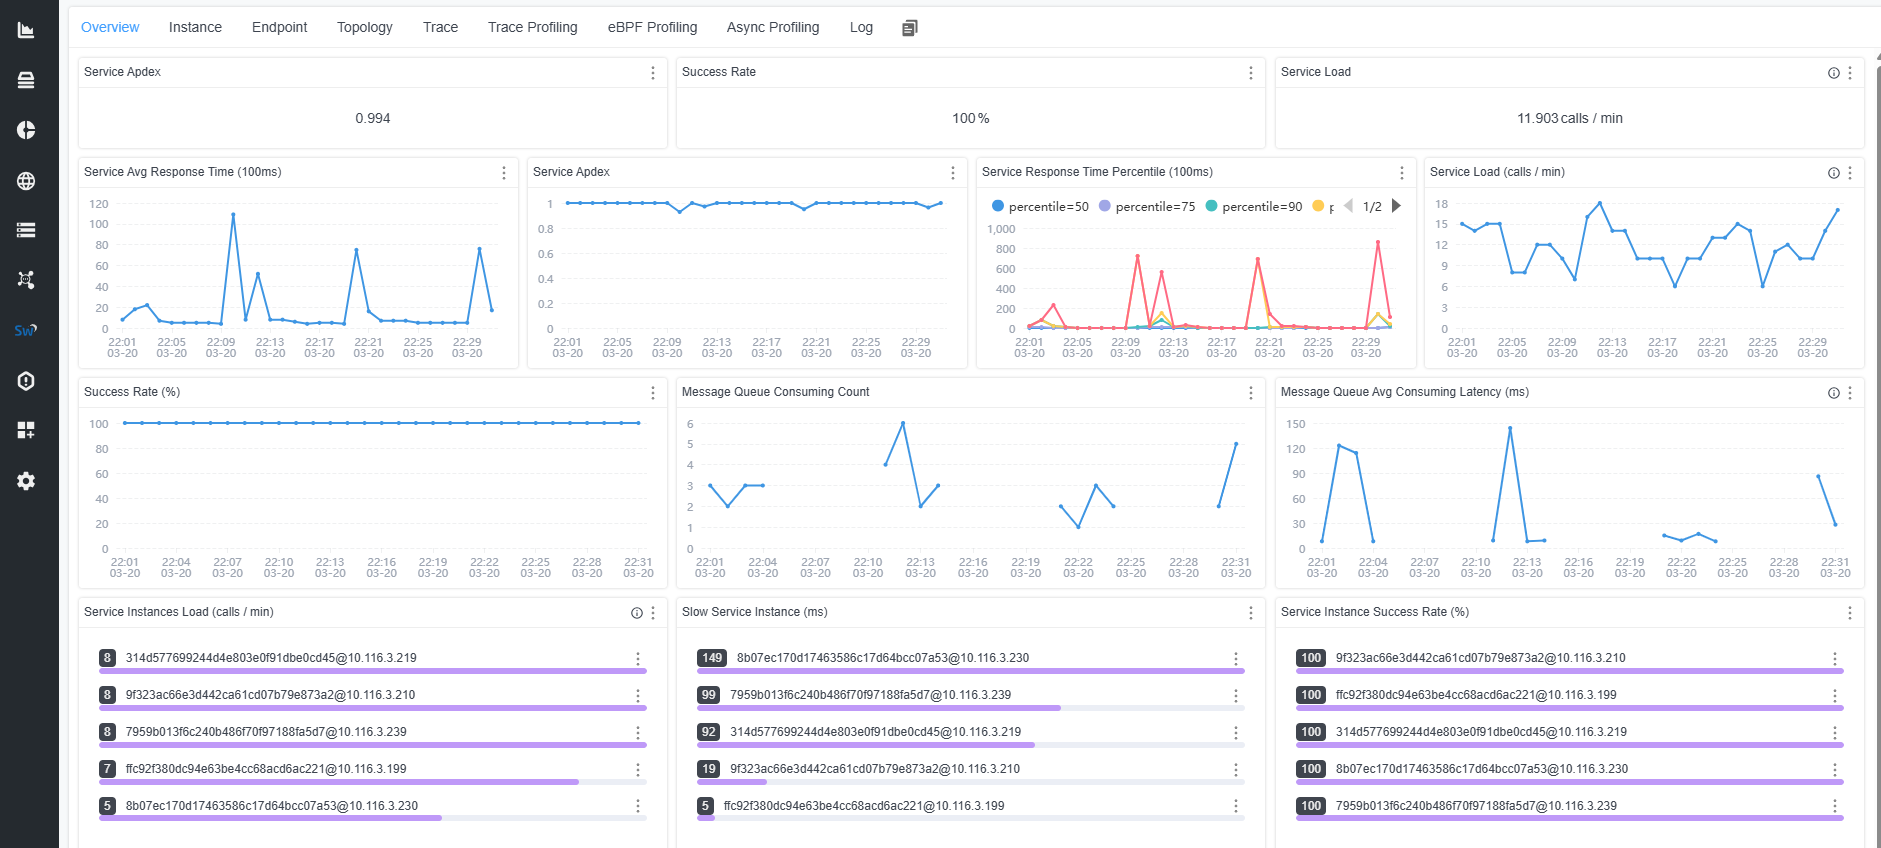
\includegraphics[width=\textwidth]{figures/SkyWalking.png}
    \caption{上传图片并提问后的效果}
    \label{fig:SkyWalking}
\end{figure}

本文使用第三章中构造的数据集作为测试数据,测试的接口为用户交互接口。在开发各个接口时,已经在各个接口上设置了监控埋点。在SkyWalking中,能够看到各个接口的
调用次数,以及接口的响应时间等信息。即便是只对某一个接口发起模拟请求,进行压力测试,也可以通过SkyWalking来查看其它所有相关接口的相关参数。
用户交互接口处于整个调用链路的起点,对其进行压测,能够观测到整个VQA系统在执行一次任务时,所有相关接口的情况,故对其进行压测。

首先,确定压测目标。本系统作为一个原型系统,拟定的用户群体规模上限在20人左右,则可以假设并发用户数目标为15人。通过对ChatGPT、DeepSeek、豆包等现有的
聊天机器人的使用的观察,发现目前普遍限制同一用户在同一时刻只能进行一个对话,若在原有对话仍在生成答案的同时,切换到新对话,将会导致原有对话的生成中断。
所以,本原型系统在压测目标上,设置每个用户的线程数都为1。
对以上各个接口,压测时长设置为30分钟。各用户线程加载,选用阶梯式加载的方式,随着时间推移,逐步增加并发用户数,以便观察系统在压力逐步增大时的性能变化。

其次,执行压测。在压测过程中,实时监控接口的性能指标,包括响应时间、吞吐量和错误率,同时监控系统的CPU使用率、内存使用率。

最终测试结果见表\ref{}。在15个并发用户下,系统响应整体较快,能满足大多数用户对视觉问答的需要。TPS表现整体稳定,错误率也比较低。总体而言,
压测结果表明,该系统能够满足其作为原型系统的要求,符合设计预期。
\begin{table}

\end{table}
\section{本章小结}

\chapter{结论与展望}
\section{本文工作总结}
本文的主要工作如下:
\begin{enumerate}[nosep]
\item 构建了一个部分可见积木世界场景空间推理VQA数据集POVQAD。
在 CLEVR 数据集的基础上,本文针对CLEVR数据集场景完全可见、不要求模型使用外部背景知识进行推理等方面的不足,构建了 POVQAD 数据集,并对其进行了统计分析和质量检验,证明了POVQAD的有效性。
\item 设计了一种规则自动补充的神经符号VQA框架RCNSP。该框架包含视觉场景理解、语义解析、迭代反馈与规则修正、
规则蒸馏、ASP推理等模块,相比现有的神经符号VQA框架,RCNSP增加了对多模态输入的支持,
并且RCNSP能够在ASP求解器进行推理前调用微调后的LLM自动对规则进行补充。
实验表明,在DeepSeek、LLaMA3、ChatGPT-4o三种LLM上,使用RCNSP比直接向VLM提问的准确率平均提升16.5\%,
比现有的神经符号VQA框架的准确率平均提升8.9\%,表明通过规则蒸馏能有效提升神经符号方法在部分可见积木世界场景中
对空间推理问答的准确率以及RCNSP在不同LLM上的泛化能力。
\item 设计实现了一个积木世界VQA系统。在RCNSP框架和POVQAD数据集基础上,设计实现了积木世界VQA原型系统,
该系统支持在针对用户的VQA任务进行空间推理时展示推理的中间步骤和逻辑链条,能够为开展自动规划教学提供辅助。
初步测试表明该系统在CPU为Intel Core i9-12900K,内存128G,显卡为3张RTX 3090并联的硬件环境下,并发量为38,
90\%响应时间为6.9秒,能够满足自动规划课堂教学场景下的用户需要。
\end{enumerate}
\section{未来工作展望}
本文所设计的RCNSP框架在支持神经符号框架的规则自动拓展、提升神经符号方法在部分可见积木世界场景下的空间推理问答准确率
方面起到了积极作用,但仍有许多方面有待完善。未来的工作可以从以下几个方面展开。

首先是迭代反馈机制的改进。目前,迭代反馈机制采用的方案是最多三轮迭代。如果在三轮迭代中,
某一轮生成的 ASP 程序能够顺利被 Clingo 执行(即不再出现语法、基础化或推理错误),
则认为程序已经达到预期的正确性,此时可以提前停止迭代。这一方案在一定程度上实现了自适应性,实现了
效率和效果之间的平衡,然而仍有进步的空间。可从以下几个方面针对该问题进行进一步研究:
\begin{enumerate}[nosep]
    \item 利用元学习或者贝叶斯优化的方法,自动搜索最优的迭代次数和反馈策略。
通过在不同任务或数据集上的交叉验证,可以自适应地调整迭代策略,使其在不同场景下达到最佳表现。
    \item 采用强化学习的方法,训练一个Agent,使其会根据当前生成 ASP 程序的状态和错误信息动态决定是否继续迭代。
类似于LLM-ARC中自动反馈调整的思路,Agent可以通过奖励信号来学习何时停止迭代,以达到最佳的平衡效果\cite{kalyanpur2024llmarcenhancingllmsautomated}。
\end{enumerate}

其次是对数据集的改进。本文构造的POVQAD数据集中,为了简化对相关问题的研究,采用 Blender 引擎渲染静态 3D 几何图像。然而目前应用领域对多模态模型的要求越来越高,静态图像为主的VQA数据集显然并不能
充分考察模型对动态空间变化的推理能力。此外,本文构造的POVQAD数据集,图像的内容是相对较为简单的几何图形,
通过脚本进行生成而得,难以模拟真实物理世界中的物体运动与视角变化等动态场景。尤其是当前智能机器人领域发展
加快,对智能体的要求越来越高,智能体需要实时理解自身运动与物体位置的关系(如“转弯后如何避开障碍物”),而静态问答无法满足需求。
可以考虑的改进方向大致有以下几点:
\begin{enumerate}[nosep]
    \item 生成动态空间问题。通过Unity或者Unreal等物理引擎的精确控制和程序化生成策略,在合成场景中模拟动态交互,自动生成涉及运动、视角变化和因果推理的动态空间问题。
    \item 增加人类视角问题。本文的POVQAD数据集中的问题,均为相机视角下的问题。可以在生成问题时,
增加更多VQA系统在图像中的人类视角的问题,以考察VQA系统在视角适应上的能力。
\end{enumerate}

\backmatter
%打印参考文献表
\thesisbib

\appendix

\end{document}
